\documentclass[aspectratio=169, professionalfonts]{beamer}
\usetheme[progressbar=frametitle]{metropolis}

\usepackage{appendixnumberbeamer}
\usepackage{booktabs}
\usepackage{caption}
\usepackage[scale=2]{ccicons}
\usepackage{outlines}
\usepackage{polyglossia}
\usepackage{subcaption}
\usepackage{unicode-math}
\usepackage{xspace}

\setmainlanguage[babelshorthands=true]{russian}
\setotherlanguage{english}
\defaultfontfeatures{Renderer=Basic, Ligatures=TeX}
\newfontfamily\cyrillicfonttt{CMU Typewriter Text}
\newfontfamily\cyrillicfont{CMU Sans Serif}
\setmainfont{CMU Sans Serif}
\setsansfont{CMU Sans Serif}
\setmonofont{CMU Typewriter Text}
\setmathfont{XITS Math}

\title{Занятие 1: Введение}
\subtitle{История вопроса и причём тут ИИ и машинное обучение}
\date{10 сентября 2022}

\begin{document}

\maketitle

\begin{frame}{Шёл 2022 год}
    \centering
    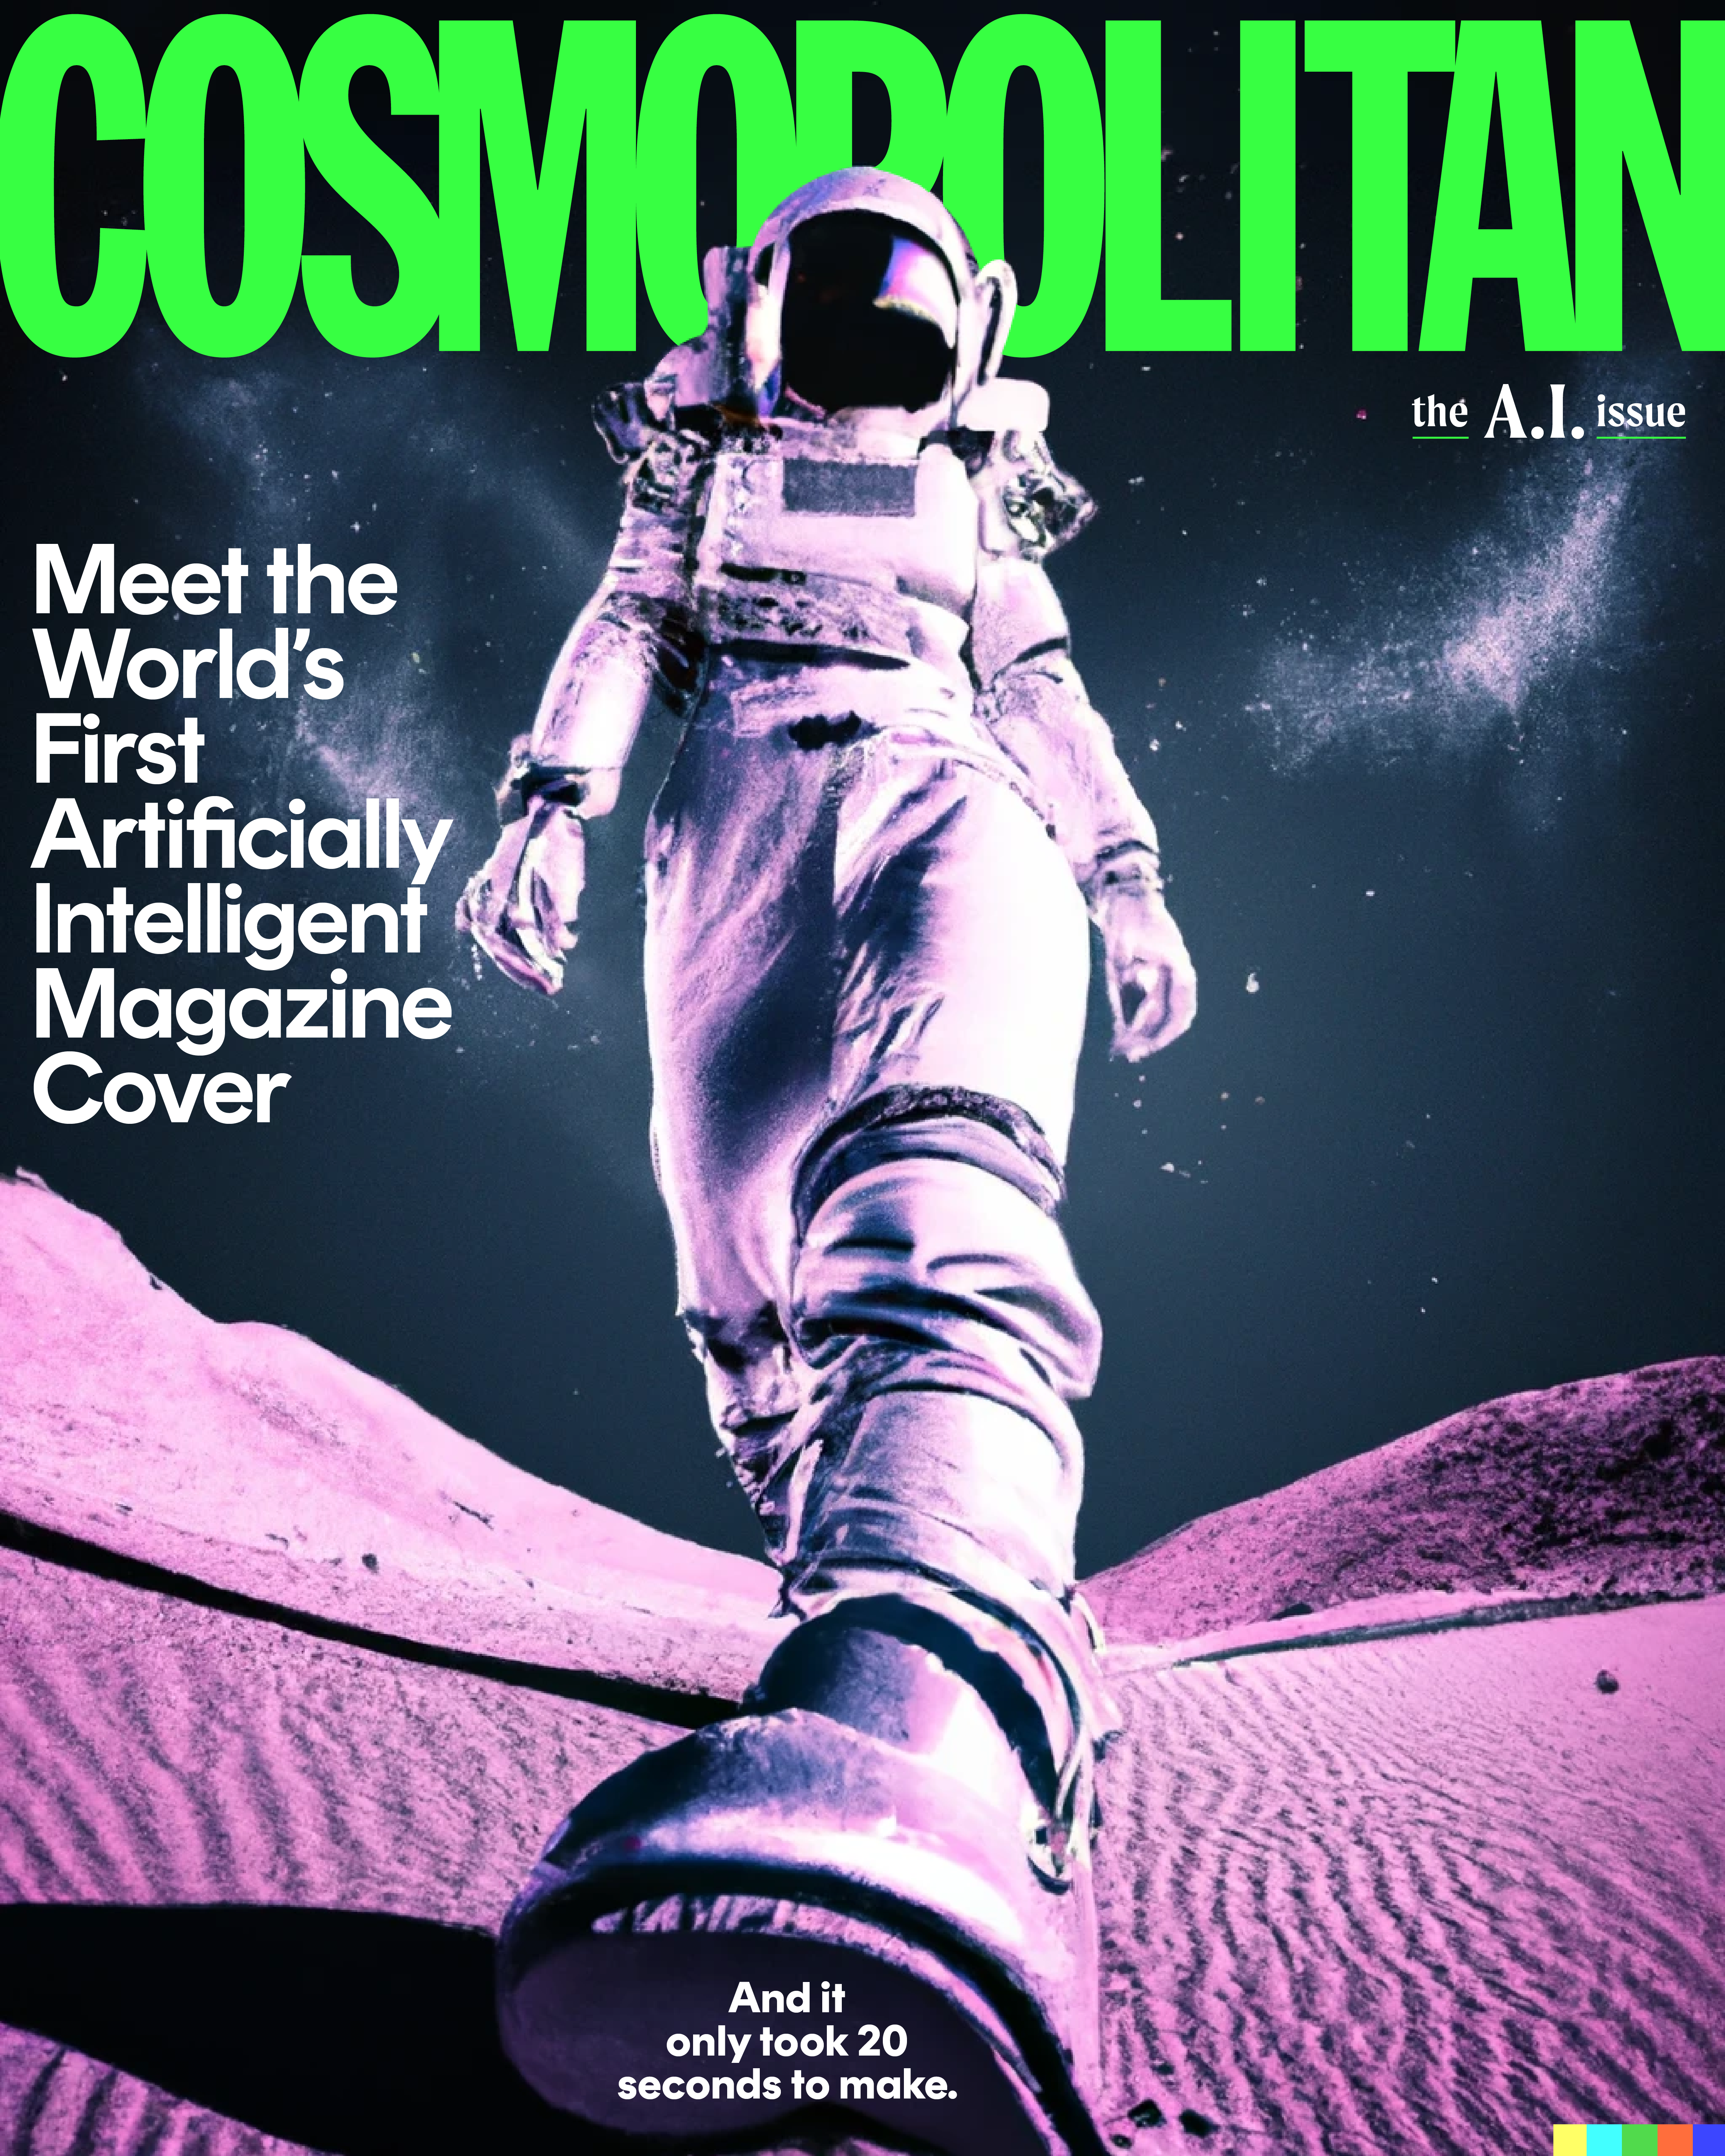
\includegraphics[width=.385\linewidth]{graphs/fig0.jpg}
\end{frame}

\begin{frame}{Шёл 2022 год}
    \centering
    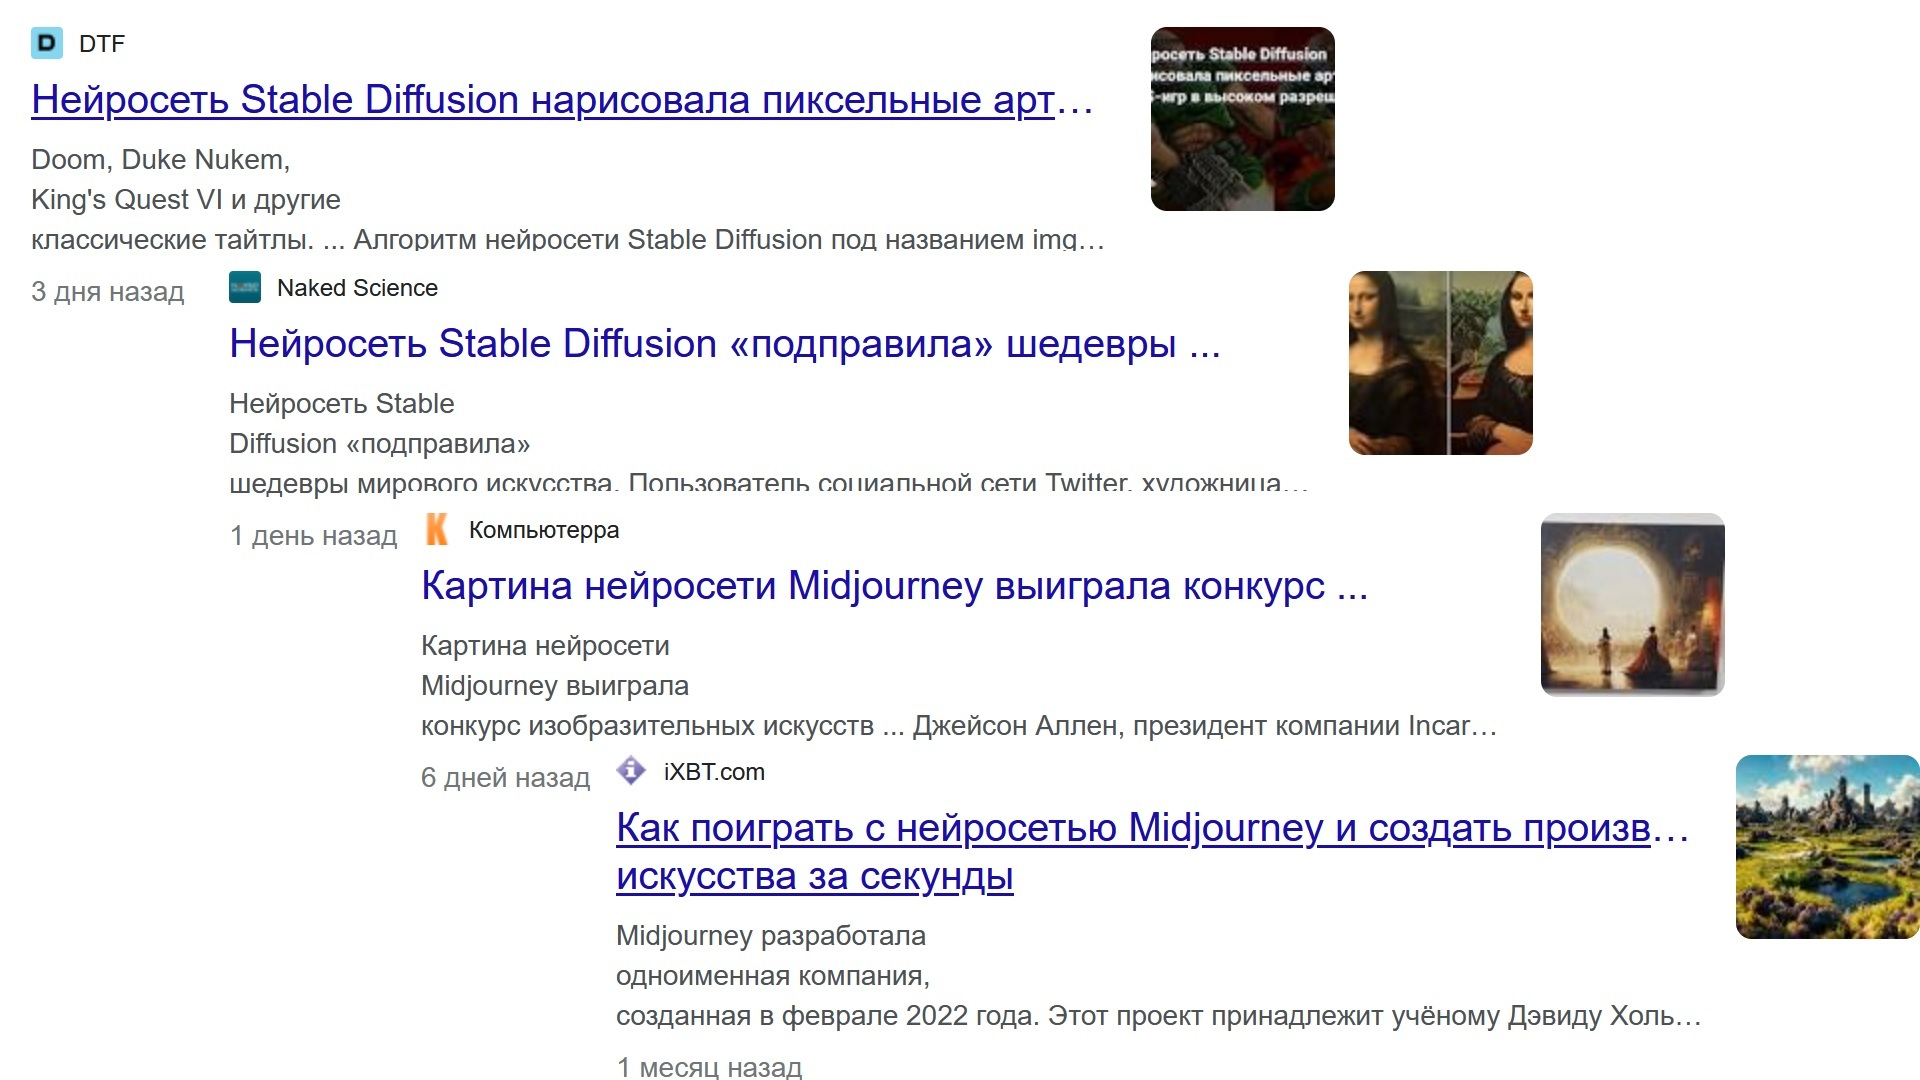
\includegraphics[width=.85\linewidth]{graphs/fig1.jpg}
\end{frame}

\begin{frame}{Шёл 2022 год}
    \centering
    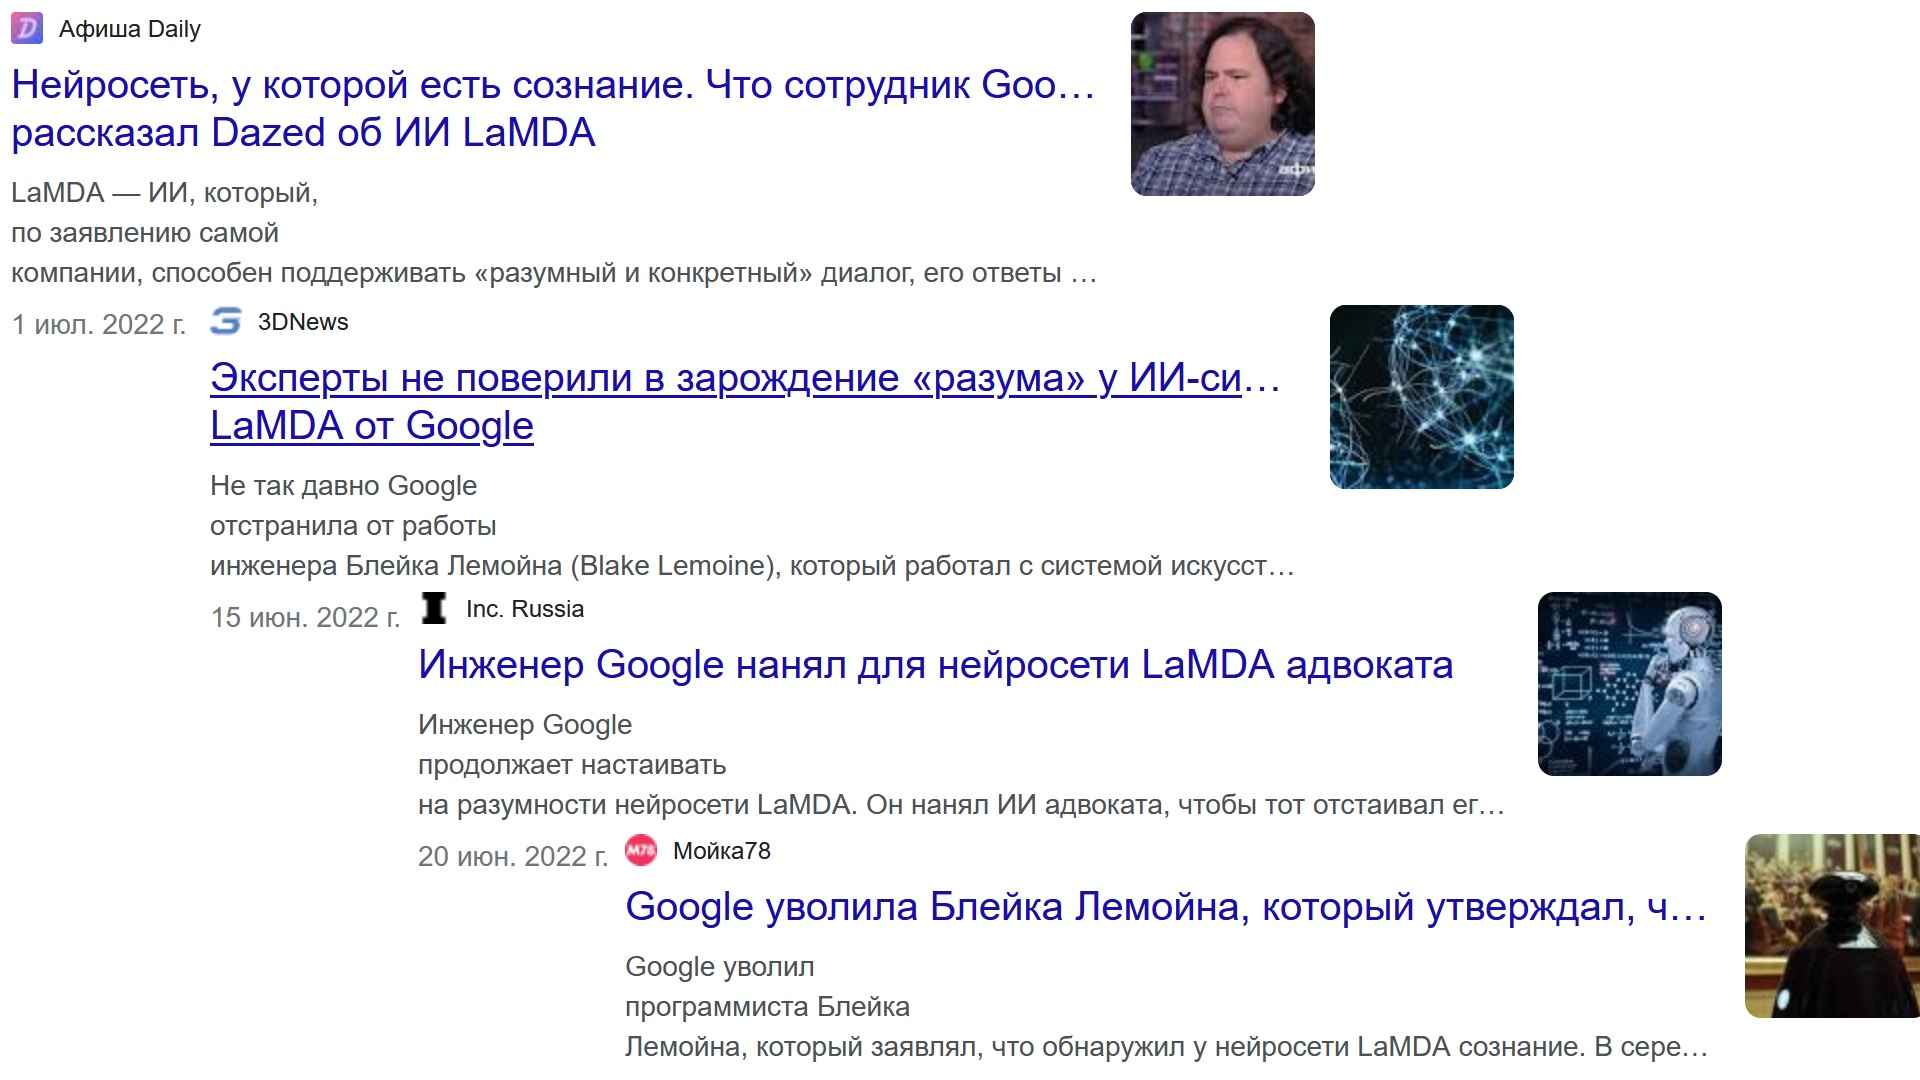
\includegraphics[width=.85\linewidth]{graphs/fig2.jpg}
\end{frame}

\begin{frame}{Кто такие нейросети и где они живут}
    \centering
    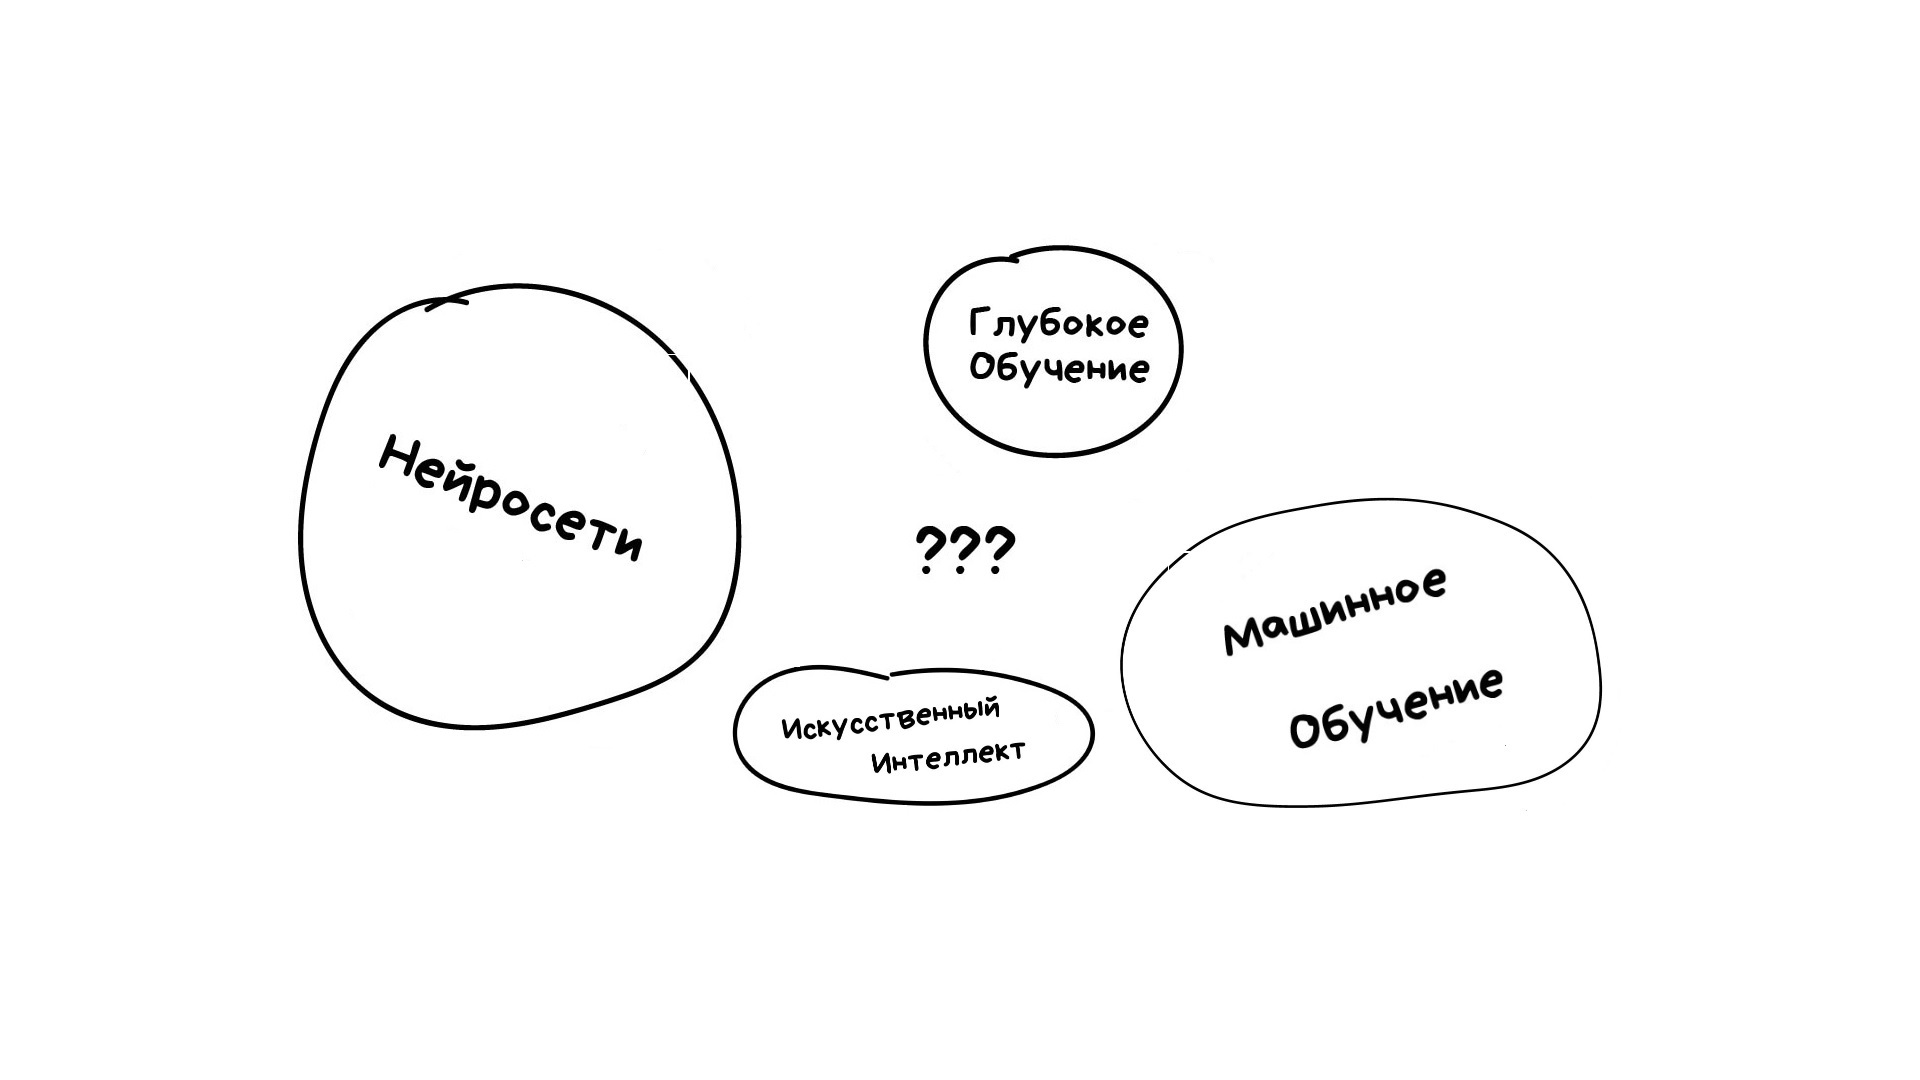
\includegraphics[width=.85\linewidth]{graphs/fig3.jpg}
\end{frame}

\begin{frame}{Кто такие нейросети и где они живут}
    Искуственный интеллект --- область науки, изучающая построение вычислимых алгоритмов для
    решения задач, которые не представляют для людей особого труда, но которые почему-то
    непонятно как запрограммировать, например:
    \begin{outline}
        \1 корректно перевести текст с одного языка на другой
        \1 диагностировать болезнь по симптомам
        \1 сказать, что изображено на картинке
        \1 порекомендовать фильм на вечер
        \1 научиться играть в го
        \1 управлять автомобилем
    \end{outline}
\end{frame}

\begin{frame}{Кто такие нейросети и где они живут}
    Разделяют сильный (strong, general) и слабый (weak) AI
    \pause
    \begin{columns}
        \begin{column}{.35\linewidth}
            \centering
            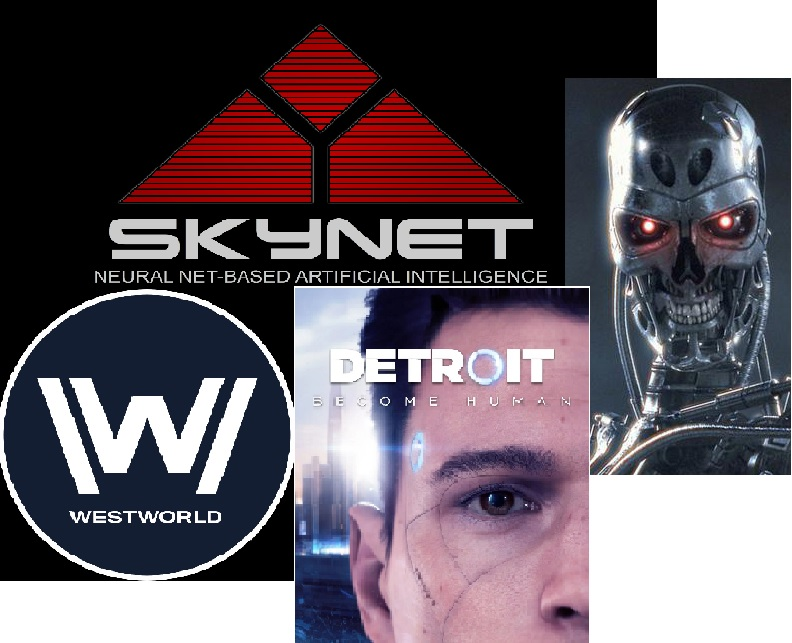
\includegraphics[width=\linewidth]{graphs/fig4_1.jpg}
            Сильный ИИ \\
            \footnotesize{захватывает человечество}
        \end{column}
        \pause
        \begin{column}{.35\linewidth}
            \centering
            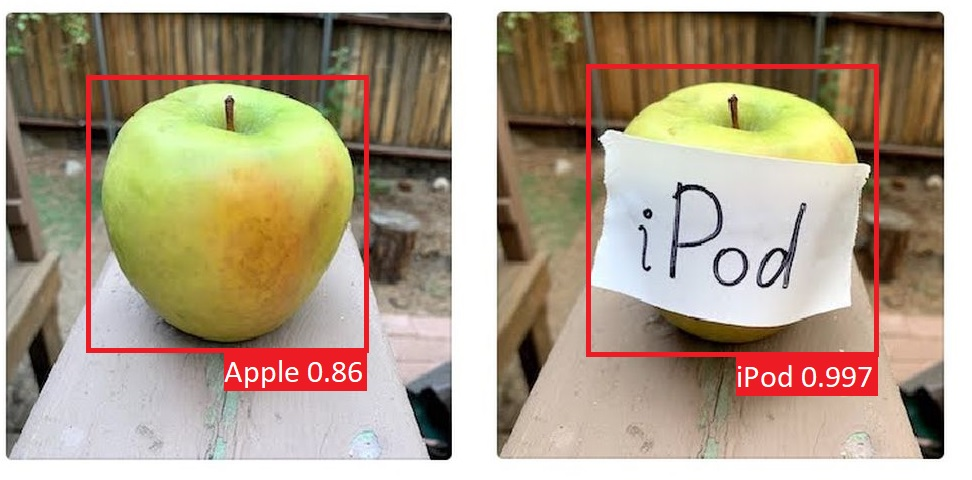
\includegraphics[width=\linewidth]{graphs/fig4_2.jpg}
            Слабый ИИ \\
            \footnotesize{превращает яблоки в iPod}
        \end{column}
    \end{columns}
\end{frame}

\begin{frame}{Кто такие нейросети и где они живут}
    Разделяют сильный (strong, general) и слабый (weak) AI:
    \begin{columns}
        \begin{column}{.35\linewidth}
            \centering
            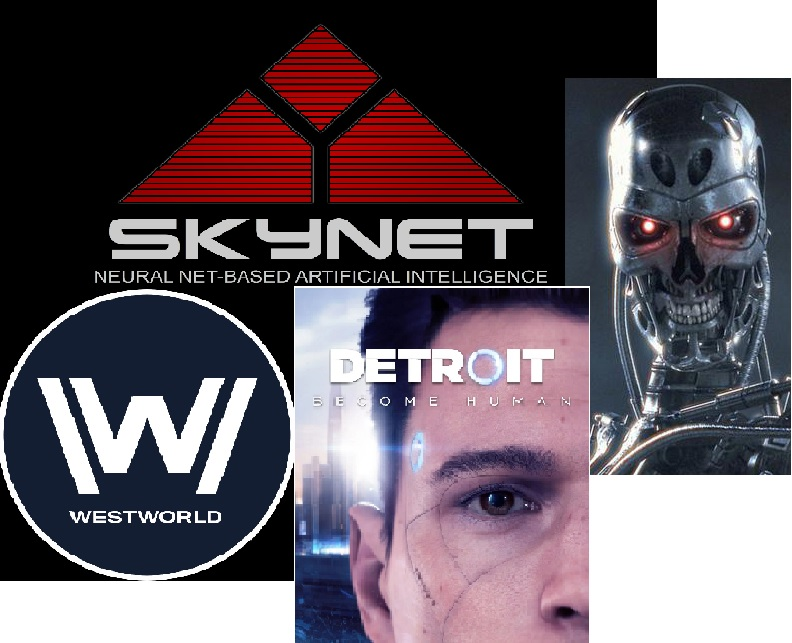
\includegraphics[width=\linewidth]{graphs/fig4_1.jpg}
            Сильный ИИ \\
            \footnotesize{полностью заменяет человека}
        \end{column}
        \begin{column}{.35\linewidth}
            \centering
            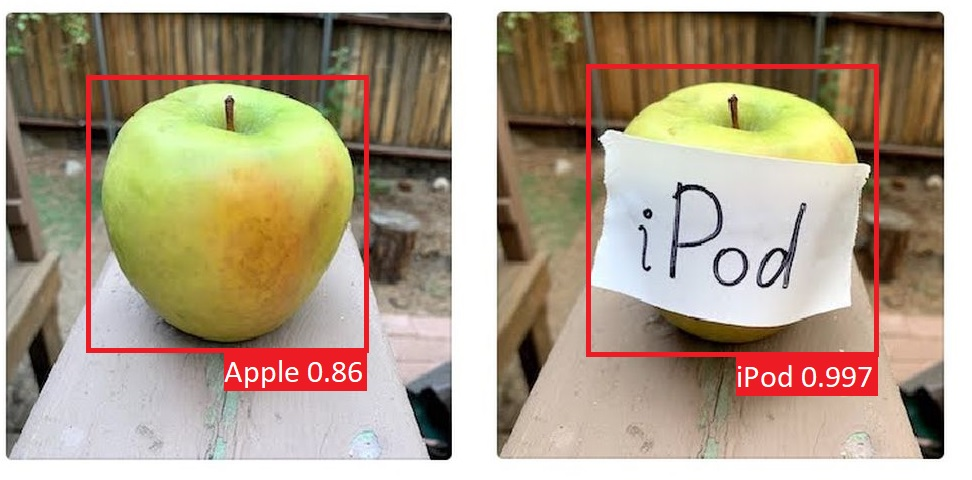
\includegraphics[width=\linewidth]{graphs/fig4_2.jpg}
            Слабый ИИ \\
            \footnotesize{решает одну узкую задачу}
        \end{column}
    \end{columns}
\end{frame}


\begin{frame}{Кто такие нейросети и где они живут}
    \begin{outline}
        \1 Машинное обучение --- область искусственного интеллекта, изучающая алгоритмы,
        автоматически улучшающися благодаря опыту
        \1 Нейронные сети --- один из множества алгоритмов машинного обучения
        \1 Глубокое обучение --- специальное название для глубоких нейронных сетей
    \end{outline}

\end{frame}

\begin{frame}{Кто такие нейросети и где они живут}
    \centering
    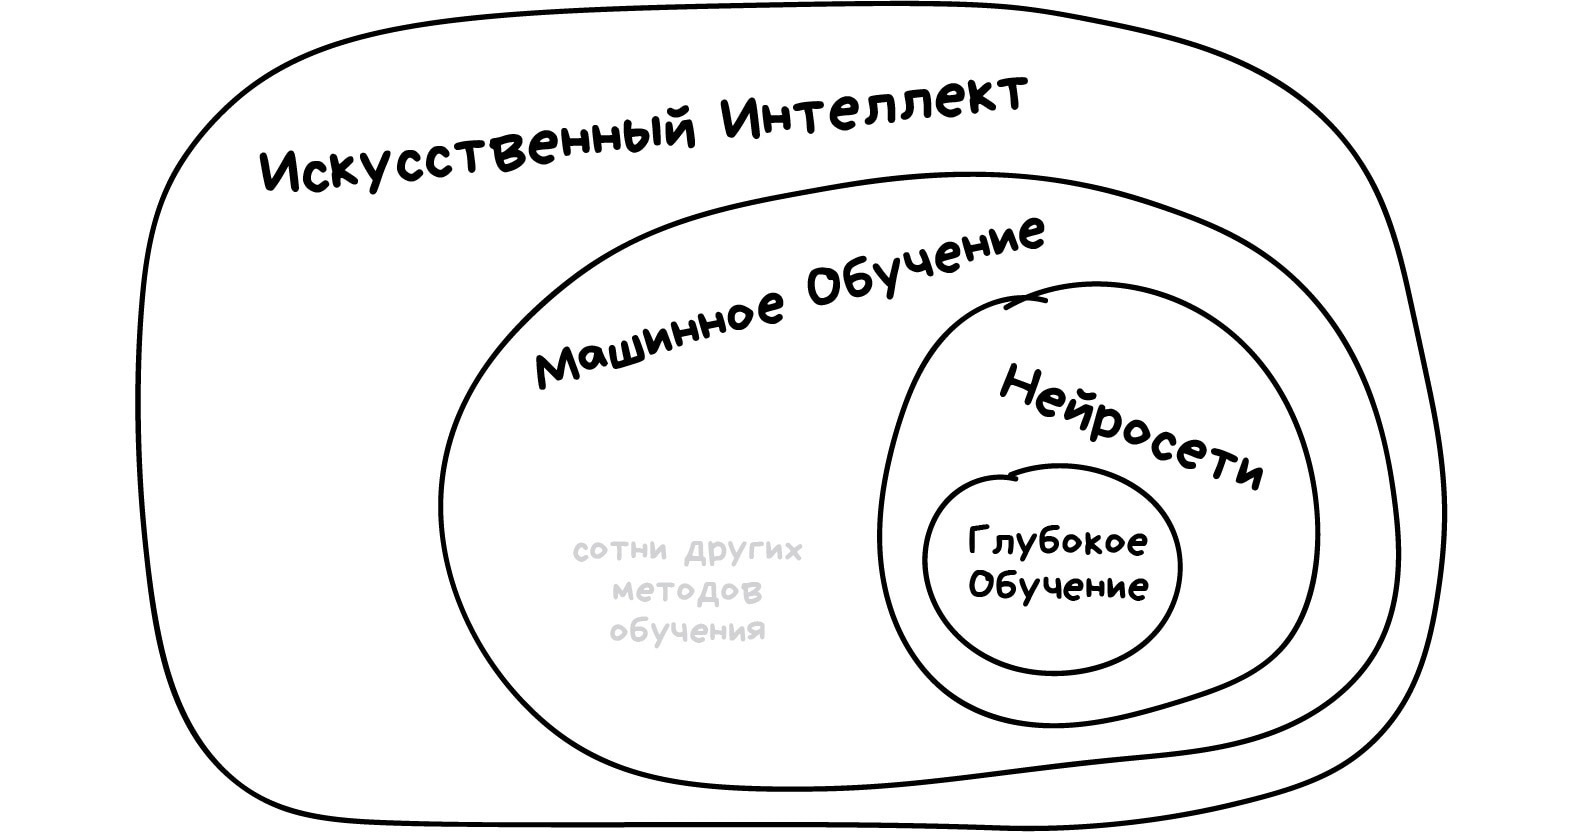
\includegraphics[width=.9\linewidth]{graphs/fig5.jpg}
\end{frame}

\begin{frame}{Особенности задач}
    \begin{outline}
        \1 корректно перевести текст с одного языка на другой
        \1 диагностировать болезнь по симптомам
        \1 сказать, что изображено на картинке
        \1 порекомендовать фильм на вечер
        \1 научиться играть в го
        \1 управлять автомобилем
    \end{outline}
\end{frame}

\begin{frame}{Особенности задач}
    Эти задачи объединяет как минимум несколько вещей:
    \begin{outline}
        \1 Их решение можно записать как функцию, которая отображает \textbf{объекты}
        (примеры, samples) в \textbf{предсказания} (targets)
            \2 \( f("Hello \ world!") \to \) "Привет, мир!"
            \2 \( f(netflix \ history) \to \) Дом Дракона --- не лучший выбор
            \2 \( f(37^\circ C) \to \) вы больны с вероятностью 0.5
        \pause
        \1 Подходит не идеальное, а достаточно хорошее решение
        \pause
        \1 Можно собрать много примеров правильных и неправильных ответов
    \end{outline}
\end{frame}

\begin{frame}{А в чём сложность?}
    \begin{columns}
        \begin{column}{.43\linewidth}
            \centering
            Ожидание в 1966
            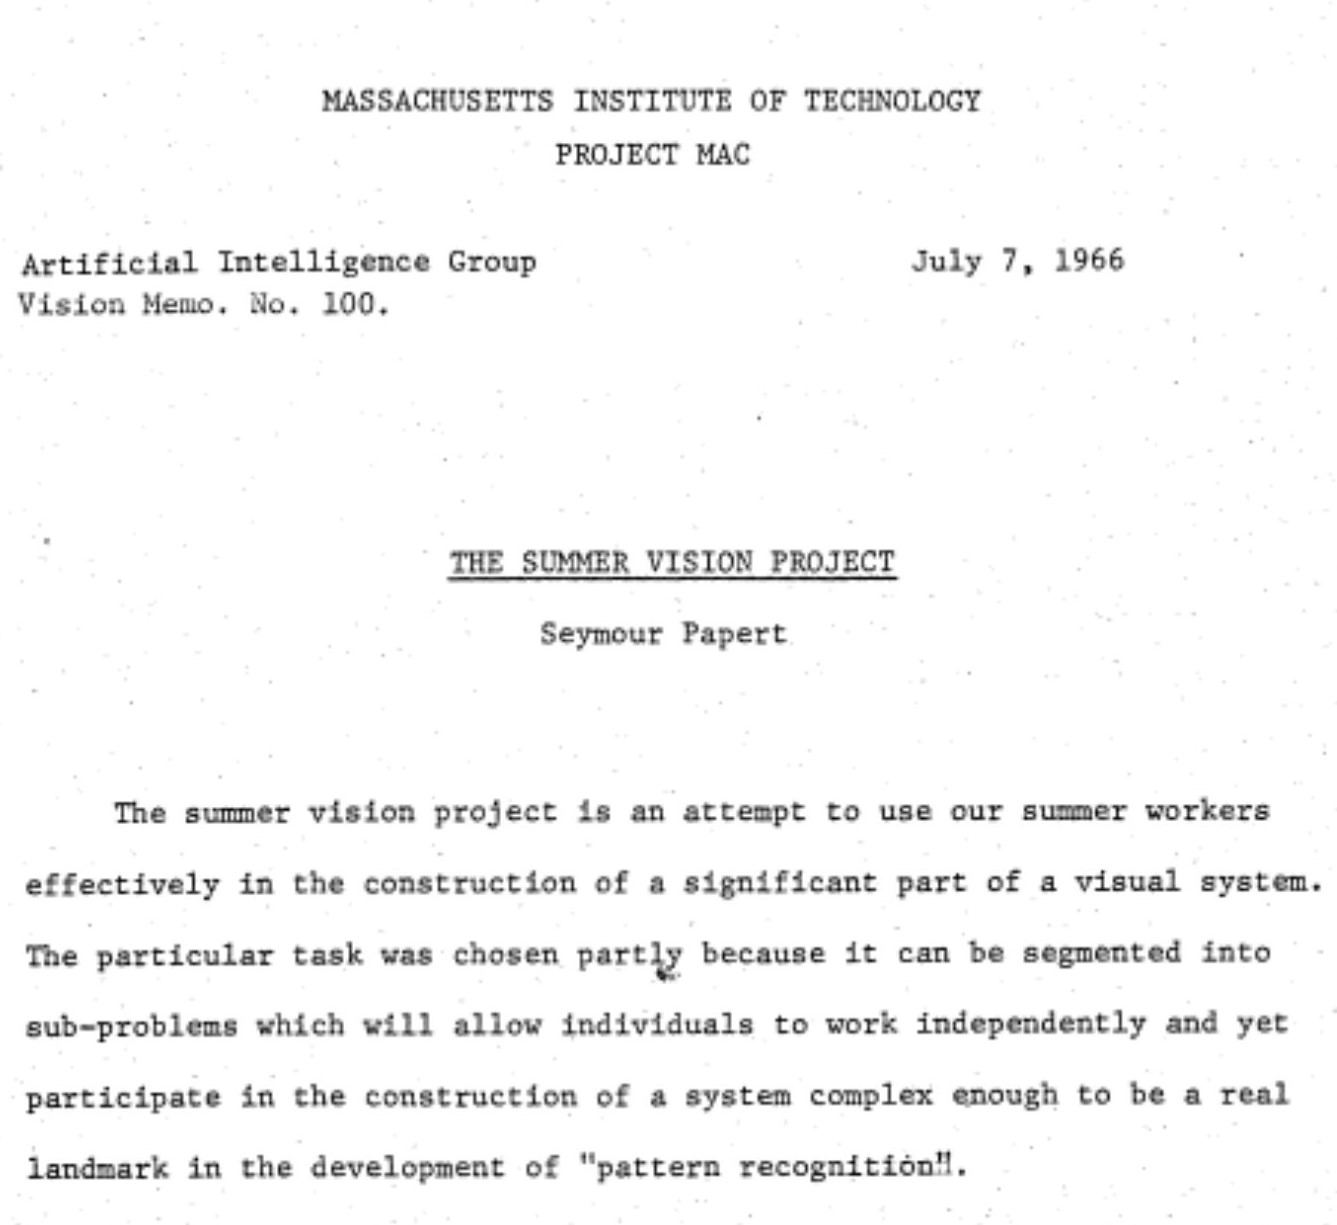
\includegraphics[width=\linewidth]{graphs/fig6_1.jpg}
        \end{column}
        \pause
        \begin{column}{.24\linewidth}
            \centering
            Реальность до 2012
            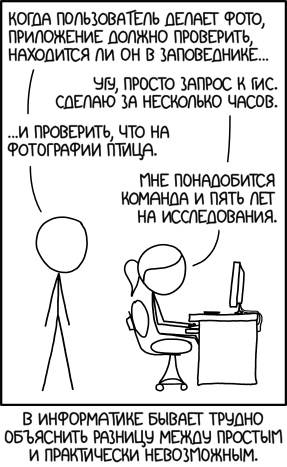
\includegraphics[width=\linewidth]{graphs/fig6_2.jpg}
        \end{column}
    \end{columns}
\end{frame}

\begin{frame}{А в чём сложность?}
    \begin{columns}
        \begin{column}{.33\linewidth}
            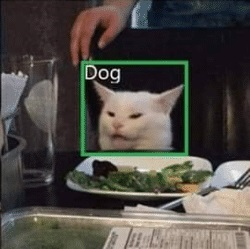
\includegraphics[width=\linewidth]{graphs/fig7_1.jpg}
        \end{column}
        \begin{column}{.33\linewidth}
            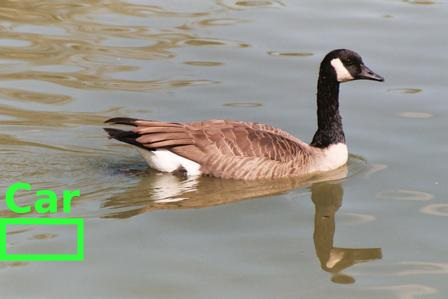
\includegraphics[width=\linewidth]{graphs/fig7_2.jpg}
        \end{column}
        \begin{column}{.33\linewidth}
            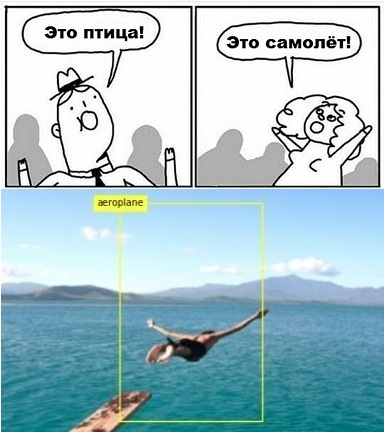
\includegraphics[width=\linewidth]{graphs/fig7_3.jpg}
        \end{column}
    \end{columns}
\end{frame}

\begin{frame}{Задача классификации изображений}
    Для заданного изображения нужно найти правильную метку
    из конечного дискретного набора \( C \)
    \vfill
    \begin{columns}
        \begin{column}{.35\linewidth}
            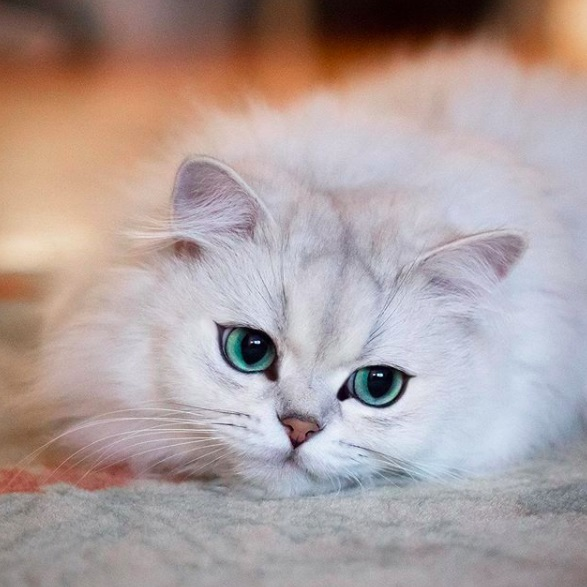
\includegraphics[width=\linewidth]{graphs/fig8.jpg}
        \end{column}
        \begin{column}{.65\linewidth}
            \( C = \{dog, cat, parrot, human, car, ninja, \ldots \} \) \\
            \hfill
            \vfill
            \( \Longrightarrow \quad \) cat
        \end{column}
    \end{columns}
\end{frame}

\begin{frame}{Задача классификации изображений}
    Более формально: построить функцию
    \( f(x) \rightarrow l, \quad l \in C \), \(x\) --- входное изображение
    \vfill
    \begin{columns}
        \begin{column}{.49\linewidth}
            \centering
            
\includegraphics[width=\linewidth]{graphs/fig9_1.jpg}
            Сортировка пузырьком
        \end{column}
        \begin{column}{.43\linewidth}
            \centering
            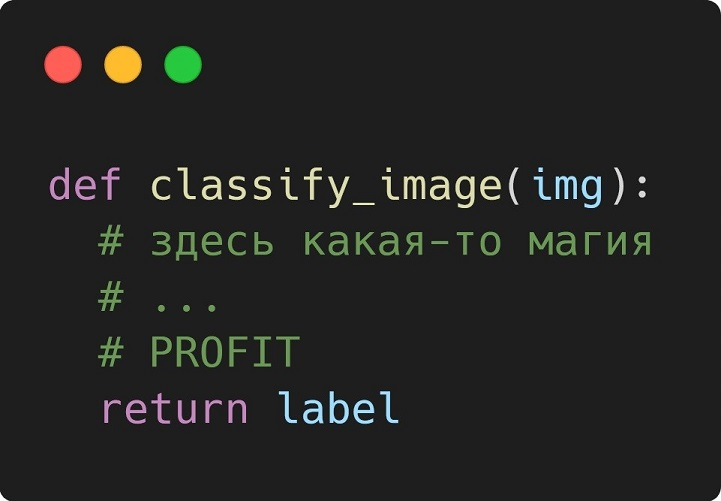
\includegraphics[width=\linewidth]{graphs/fig9_2.jpg}
            Классификация
        \end{column}
    \end{columns}
\end{frame}

\begin{frame}{Проблема: семантический разрыв (semantic gap)}
    \begin{columns}
        \begin{column}{.35\linewidth}
            \centering
            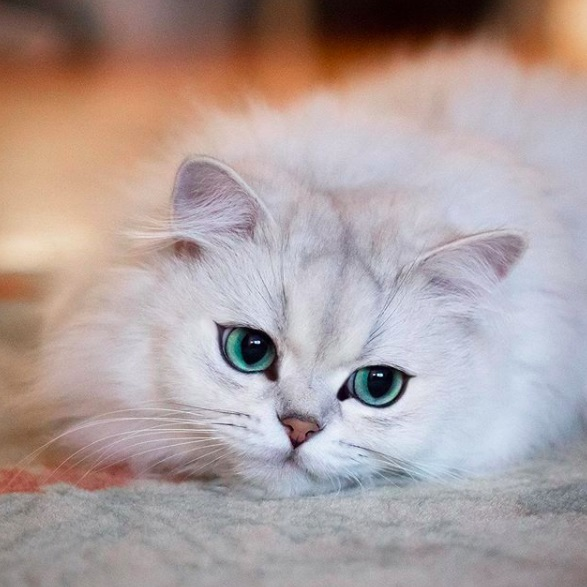
\includegraphics[width=\linewidth]{graphs/fig8.jpg}
            Что видим мы: кошка
        \end{column}
        \pause
        \begin{column}{.65\linewidth}
            \centering
            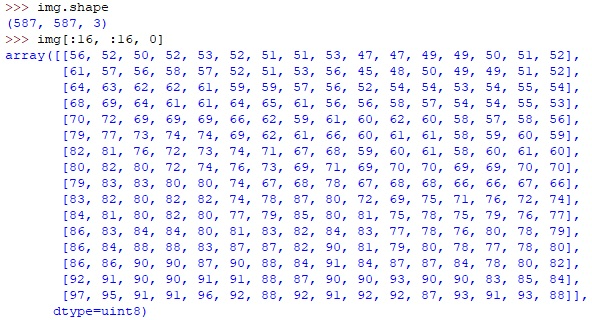
\includegraphics[width=\linewidth]{graphs/fig10.jpg}
            Что видит компьютер: WTF?
        \end{column}
    \end{columns}
\end{frame}

\begin{frame}{Проблемы: смена ракурса}
    \begin{columns}
        \begin{column}{.325\linewidth}
            \centering
            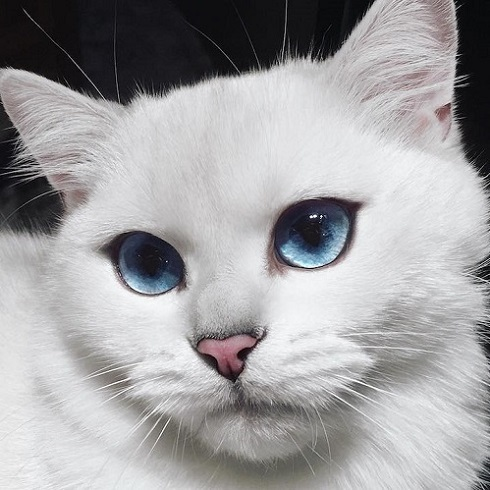
\includegraphics[width=\linewidth]{graphs/fig11_1.jpg}
        \end{column}
        \begin{column}{.325\linewidth}
            \centering
            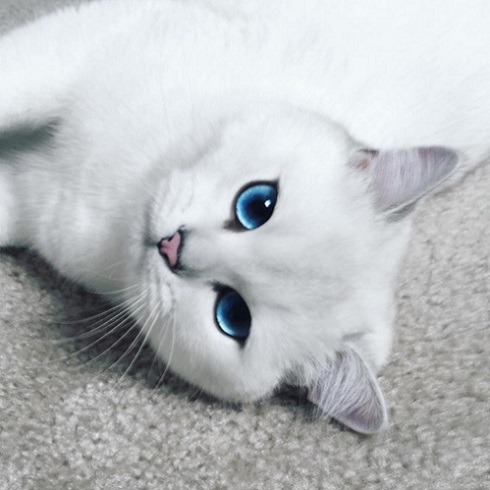
\includegraphics[width=\linewidth]{graphs/fig11_2.jpg}
        \end{column}
        \begin{column}{.325\linewidth}
            \centering
            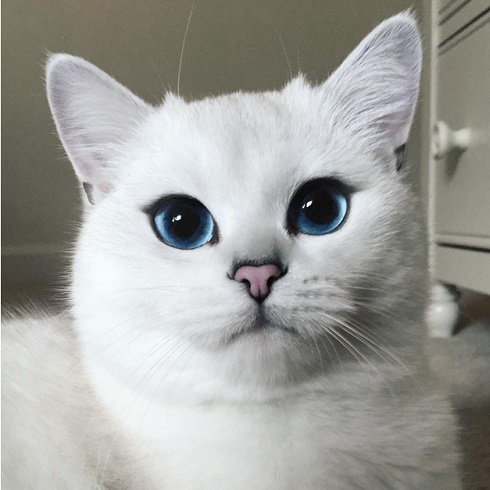
\includegraphics[width=\linewidth]{graphs/fig11_3.jpg}
        \end{column}
    \end{columns}
\end{frame}

\begin{frame}{Проблемы: разное освещение}
    \begin{columns}
        \begin{column}{.325\linewidth}
            \centering
            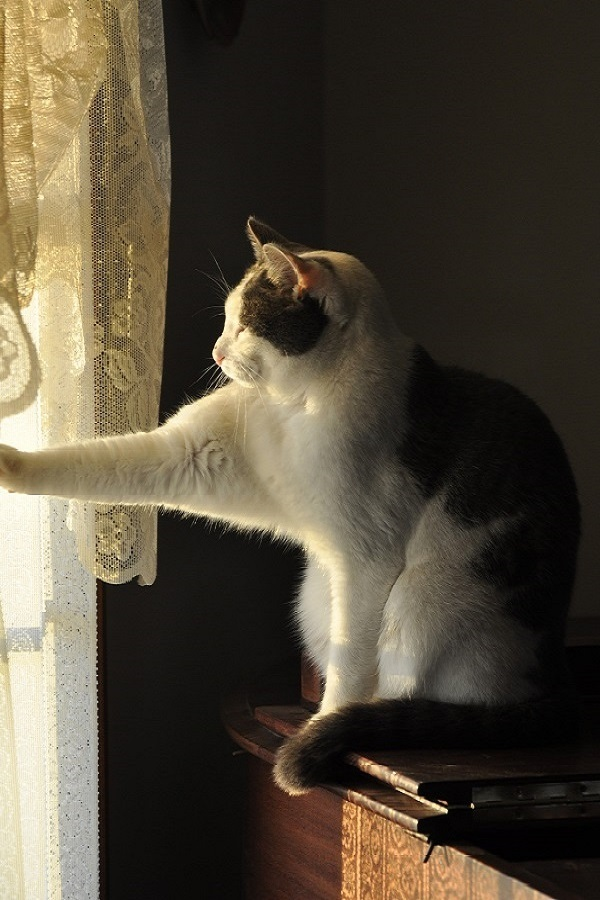
\includegraphics[width=\linewidth]{graphs/fig12_1.jpg}
        \end{column}
        \begin{column}{.325\linewidth}
            \centering
            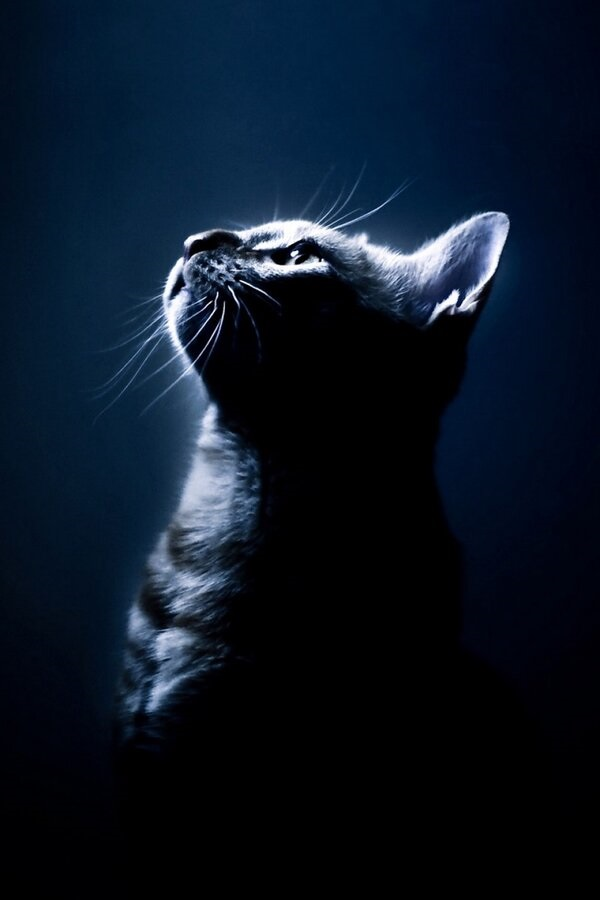
\includegraphics[width=\linewidth]{graphs/fig12_2.jpg}
        \end{column}
        \begin{column}{.325\linewidth}
            \centering
            
\includegraphics[width=\linewidth]{graphs/fig12_3.jpg}
        \end{column}
    \end{columns}
\end{frame}

\begin{frame}{Сложности: вариация форм (коты жидкие)}
    \begin{columns}
        \begin{column}{.325\linewidth}
            \centering
            
\includegraphics[width=\linewidth]{graphs/fig13_1.jpg}
        \end{column}
        \begin{column}{.325\linewidth}
            \centering
            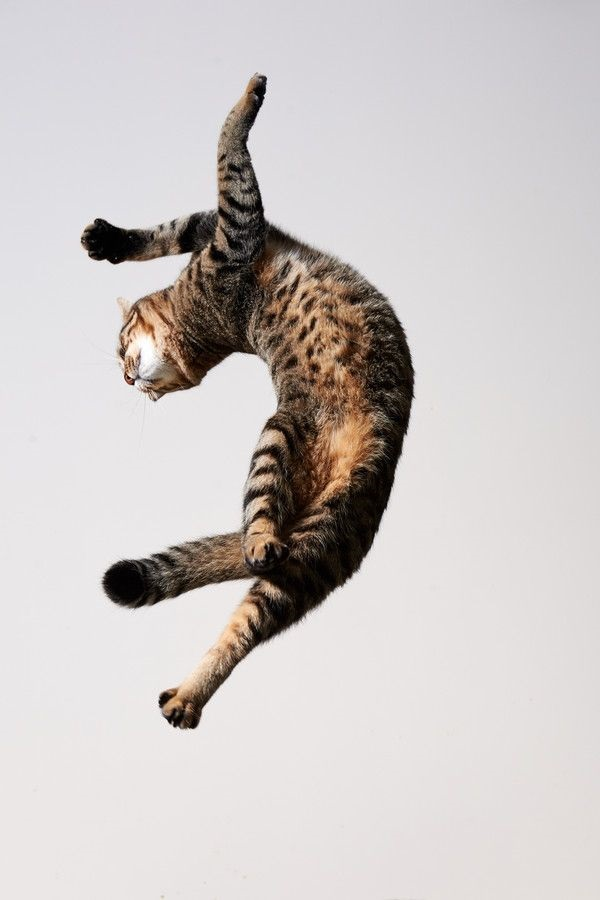
\includegraphics[width=\linewidth]{graphs/fig13_2.jpg}
        \end{column}
        \begin{column}{.325\linewidth}
            \centering
            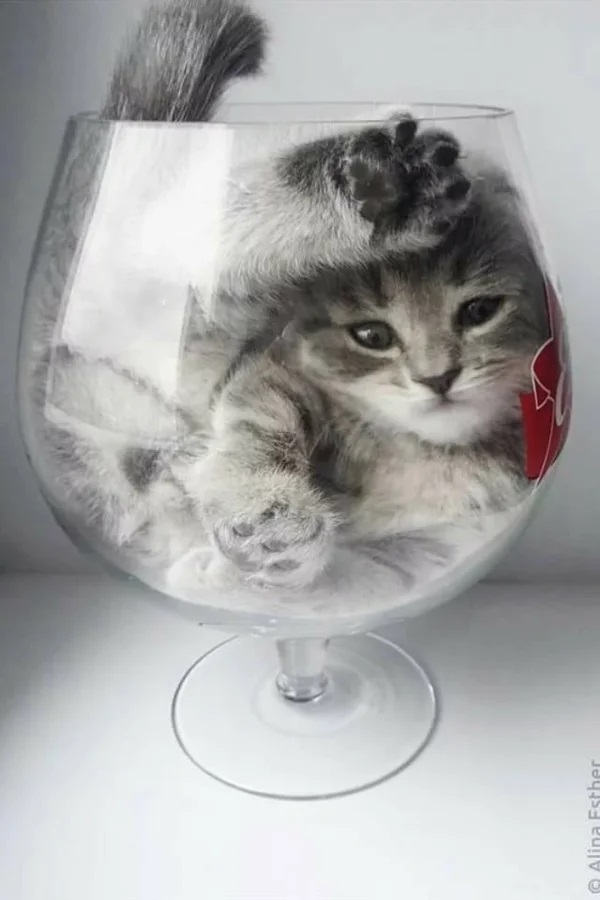
\includegraphics[width=\linewidth]{graphs/fig13_3.jpg}
        \end{column}
    \end{columns}
\end{frame}

\begin{frame}{Сложности: внутриклассовая вариативность}
    \centering
    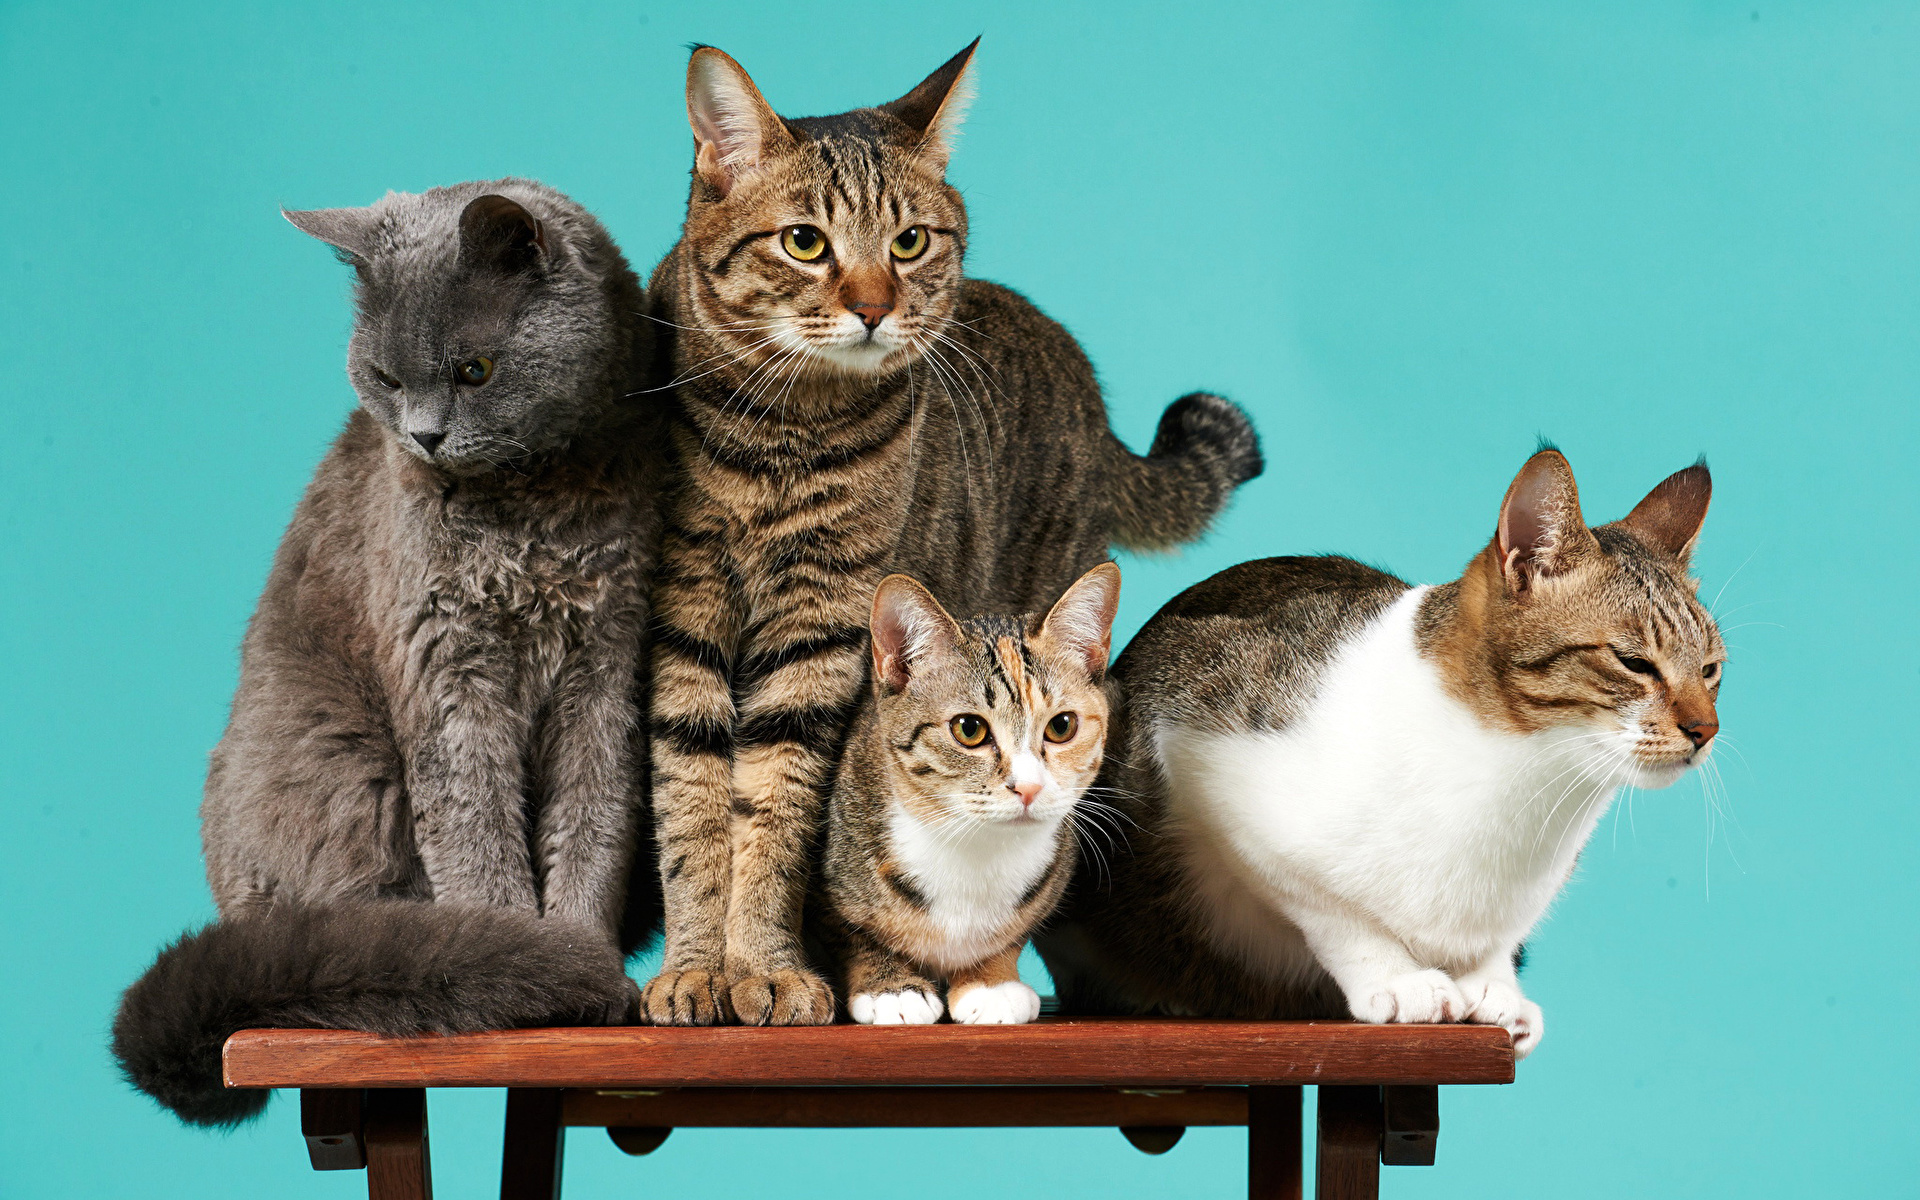
\includegraphics[width=.77\linewidth]{graphs/fig14.jpg}
\end{frame}

\begin{frame}{Поражение алгоритмов}
    \centering
    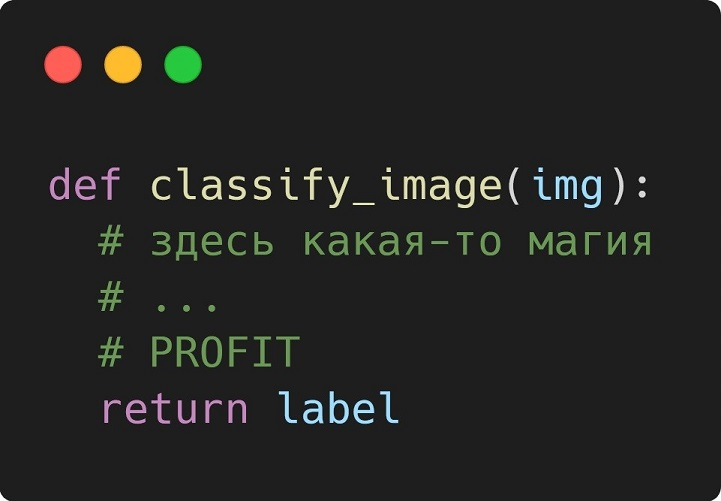
\includegraphics[width=.5\linewidth]{graphs/fig9_2.jpg}

    \textbf{Простого} способа построить такую функцию так и не нашлось
\end{frame}

\begin{frame}{Поражение алгоритмов}
    Конечно, было предпринято множество попыток, например
    \vfill
    \begin{columns}
        \begin{column}{.25\linewidth}
            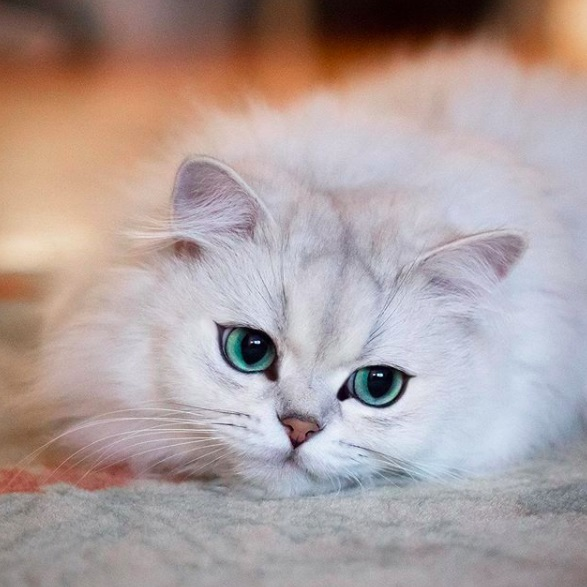
\includegraphics[width=\linewidth]{graphs/fig8.jpg}
        \end{column}
        \begin{column}{.15\linewidth}
            \centering
            \( \longrightarrow \) \\
            границы
        \end{column}
        \begin{column}{.25\linewidth}
            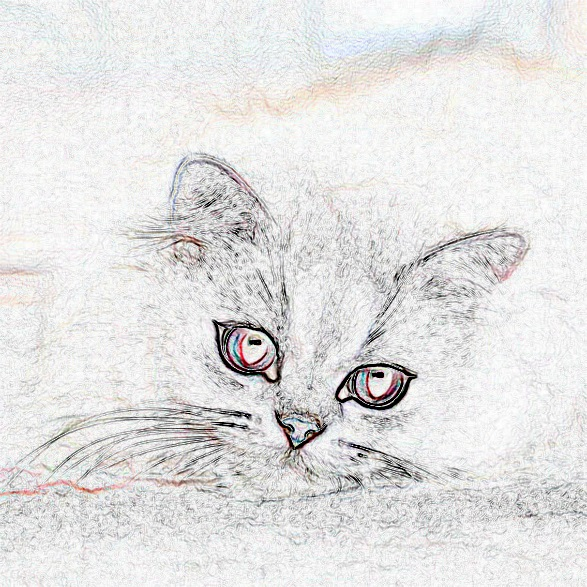
\includegraphics[width=\linewidth]{graphs/fig15_1.jpg}
        \end{column}
        \begin{column}{.15\linewidth}
            \centering
            \( \longrightarrow \) \\
            углы
        \end{column}
        \begin{column}{.07\linewidth}
            
\includegraphics[width=\linewidth]{graphs/fig15_2.jpg}
        \end{column}
        \begin{column}{.13\linewidth}
            \centering
            \( \longrightarrow  \) \\
            \(? \)
        \end{column}
    \end{columns}
\end{frame}

\begin{frame}{A wild data driven machine learning appears}
    \centering
    
\includegraphics[width=.73\linewidth]{graphs/fig16.jpg}
\end{frame}

\begin{frame}{Терминология машинного обучения}
    \begin{outline}
        \1 Машинное обучение изучает алгоритмы, улучшающися благодаря опыту
        \1 Функция --- \textbf{модель}
        \1 Набор примеров --- \textbf{обучающия выборка, датасет}
            \2 объекты (\textbf{семплы}) + ответы (\textbf{таргеты})
    \end{outline}
    \begin{columns}
        \begin{column}{.1\linewidth}
            \centering
            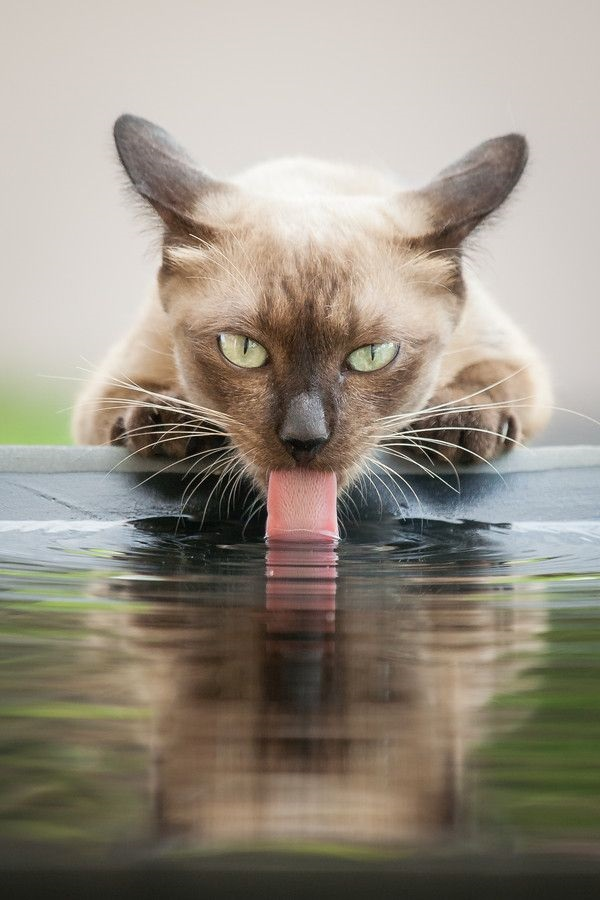
\includegraphics[width=\linewidth]{graphs/fig17_1.jpg}
            `cat'
        \end{column}
        \begin{column}{.1\linewidth}
            \centering
            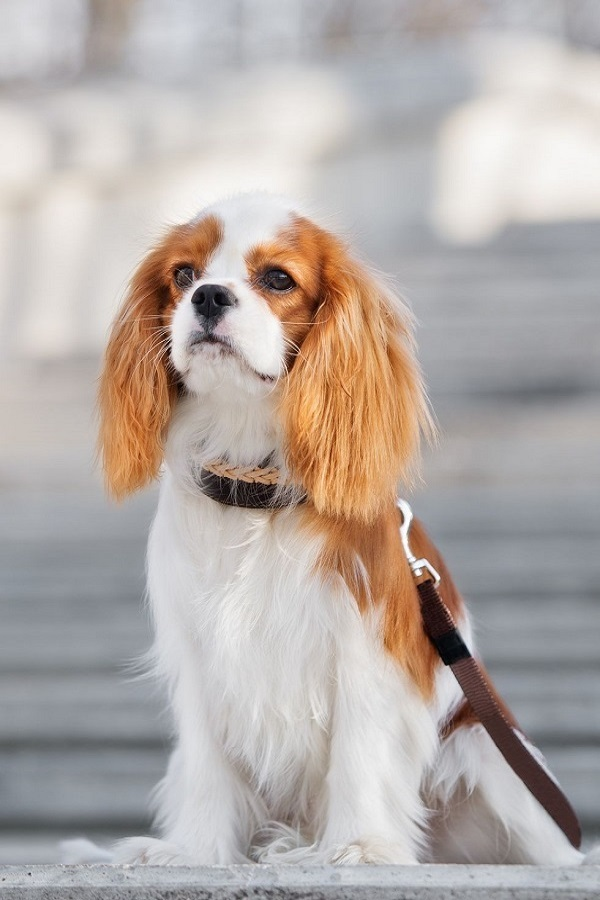
\includegraphics[width=\linewidth]{graphs/fig17_2.jpg}
            `dog'
        \end{column}
        \begin{column}{.1\linewidth}
            \centering
            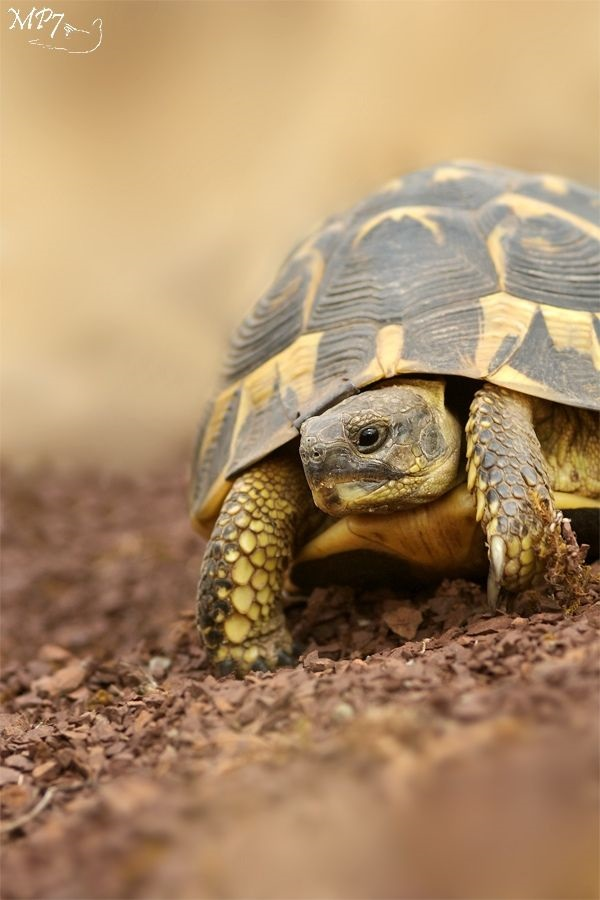
\includegraphics[width=\linewidth]{graphs/fig17_3.jpg}
            `ninja'
        \end{column}
        \begin{column}{.1\linewidth}
            \centering
            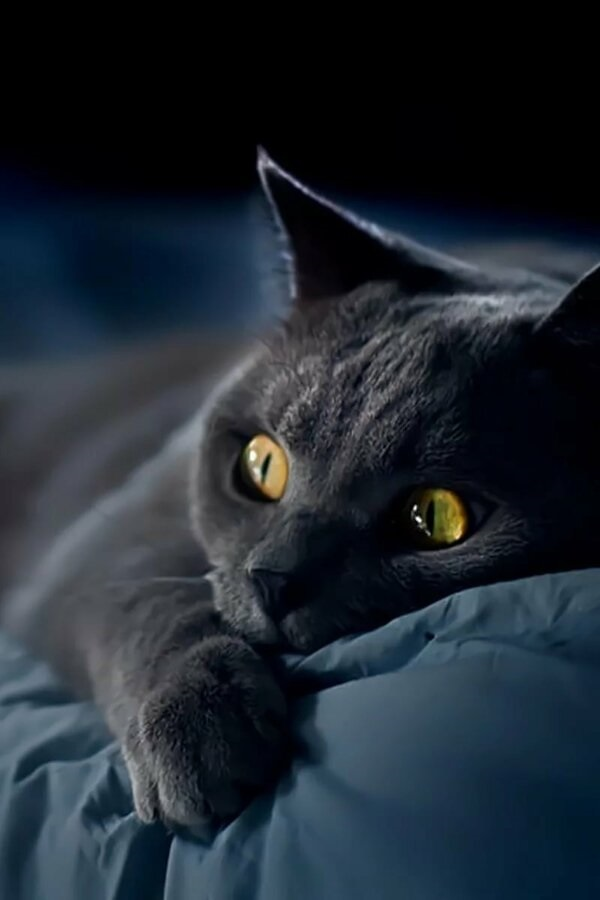
\includegraphics[width=\linewidth]{graphs/fig17_4.jpg}
            `cat'
        \end{column}
        \begin{column}{.1\linewidth}
            \centering
            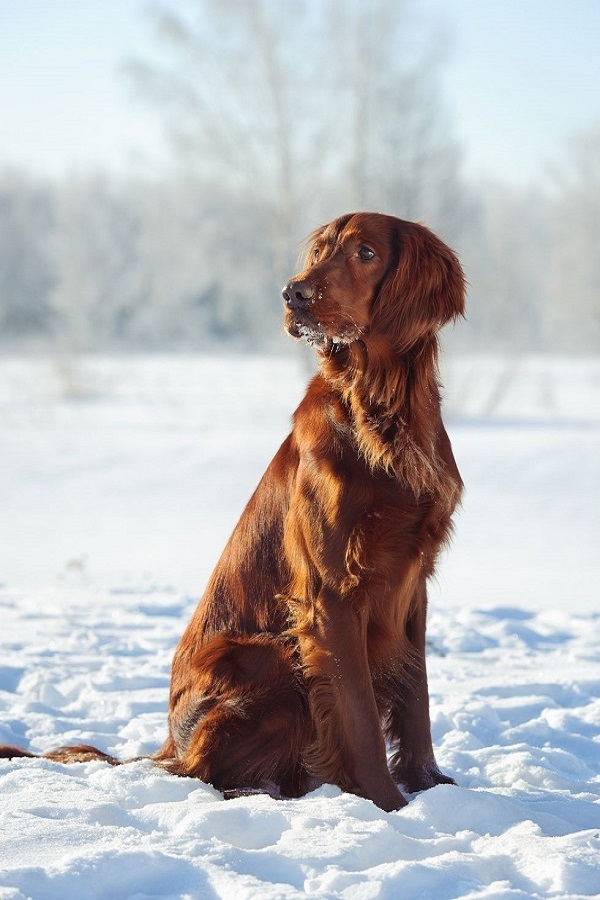
\includegraphics[width=\linewidth]{graphs/fig17_5.jpg}
            `dog'
        \end{column}
        \begin{column}{.1\linewidth}
            \centering
            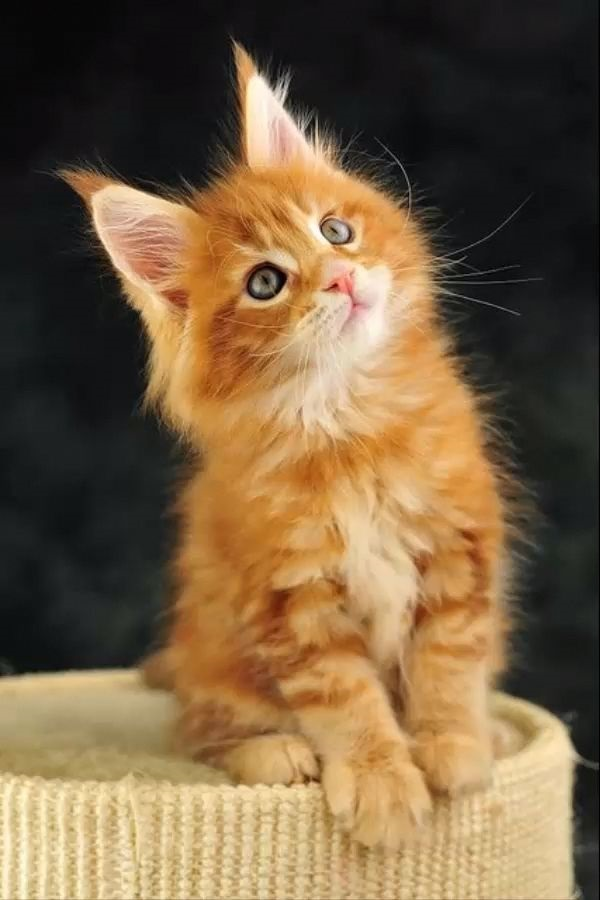
\includegraphics[width=\linewidth]{graphs/fig17_6.jpg}
            `cat'
        \end{column}
        \begin{column}{.1\linewidth}
            \centering
            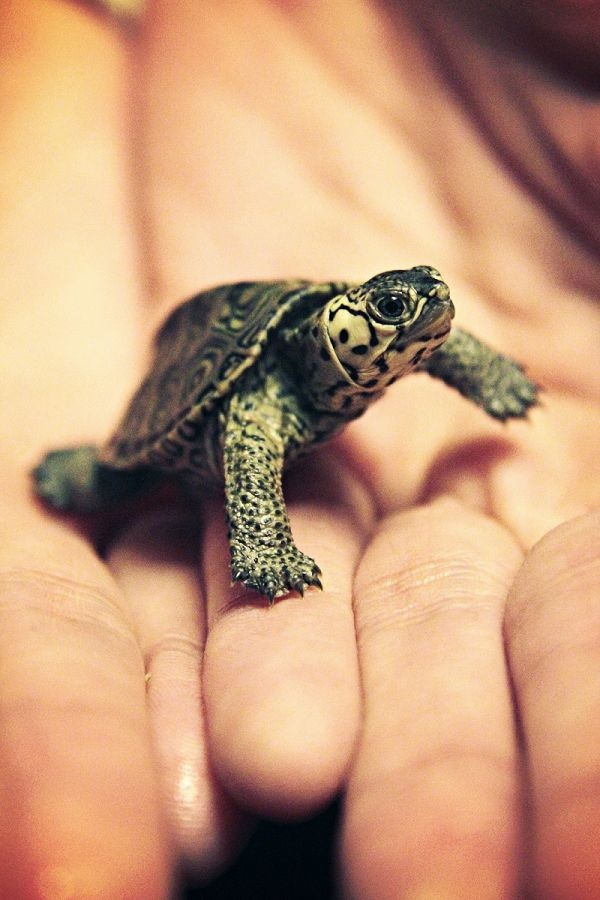
\includegraphics[width=\linewidth]{graphs/fig17_7.jpg}
            `ninja'
        \end{column}
        \begin{column}{.1\linewidth}
            \centering
            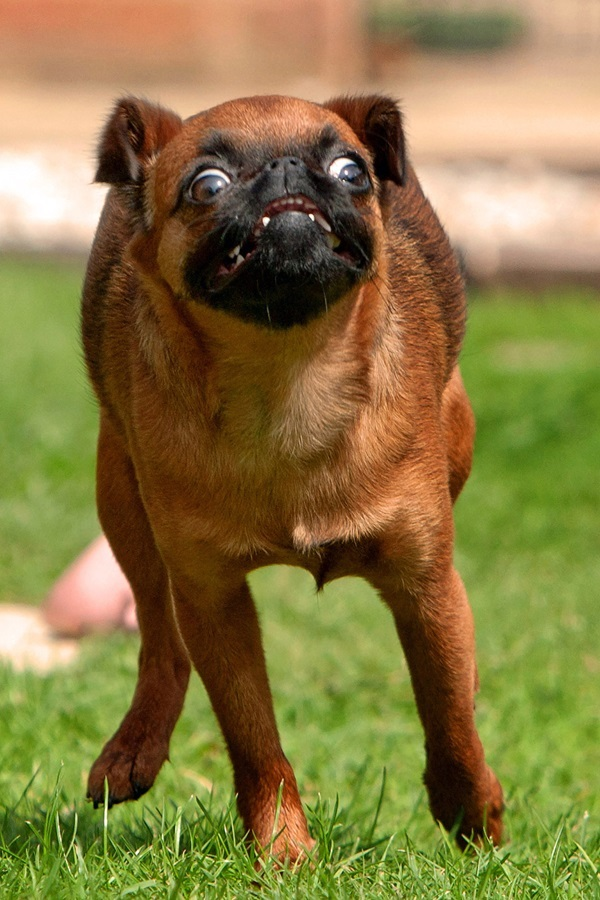
\includegraphics[width=\linewidth]{graphs/fig17_8.jpg}
            `dog'
        \end{column}
        \begin{column}{.1\linewidth}
            \centering
            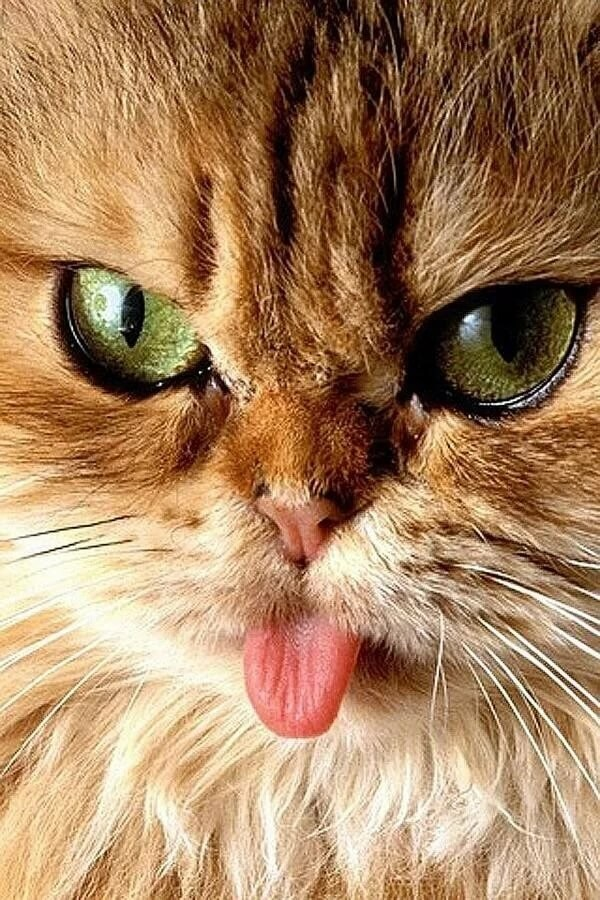
\includegraphics[width=\linewidth]{graphs/fig17_9.jpg}
            `cat'
        \end{column}
    \end{columns}
\end{frame}

\begin{frame}{Машинное обучение: data driven}
    \centering
    Теперь наша функция превращается в две:
    \begin{columns}[T]
        \begin{column}{.4\linewidth}
            \centering
            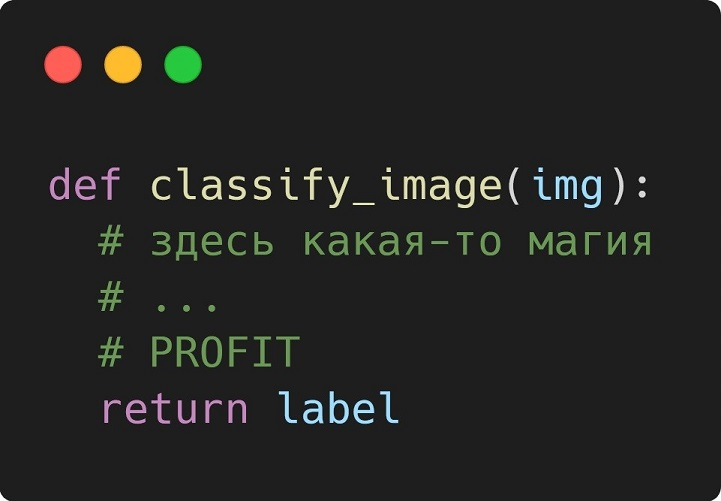
\includegraphics[width=\linewidth]{graphs/fig9_2.jpg}
        \end{column}
        \begin{column}{.6\linewidth}
            \centering
            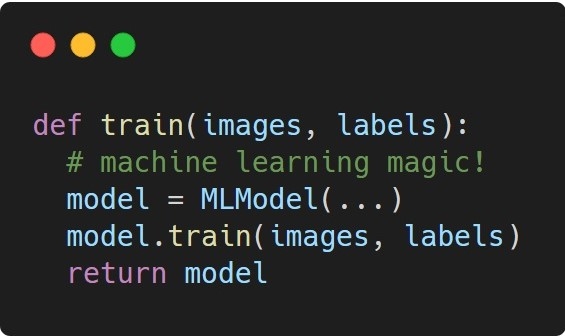
\includegraphics[width=.64\linewidth]{graphs/fig18_1.jpg}
            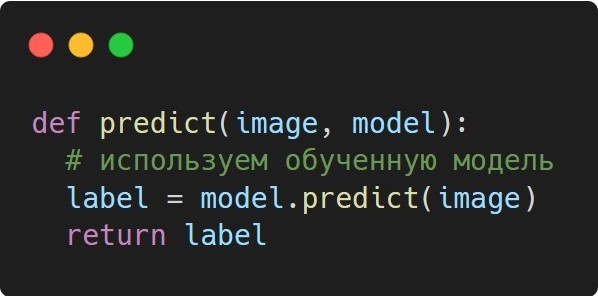
\includegraphics[width=.64\linewidth]{graphs/fig18_2.jpg}
        \end{column}
    \end{columns}
\end{frame}

\begin{frame}{Computer Science vs. ML}
    \begin{columns}[T]
        \begin{column}{.49\linewidth}
            \centering
            Computer Science \& Software Engineering
            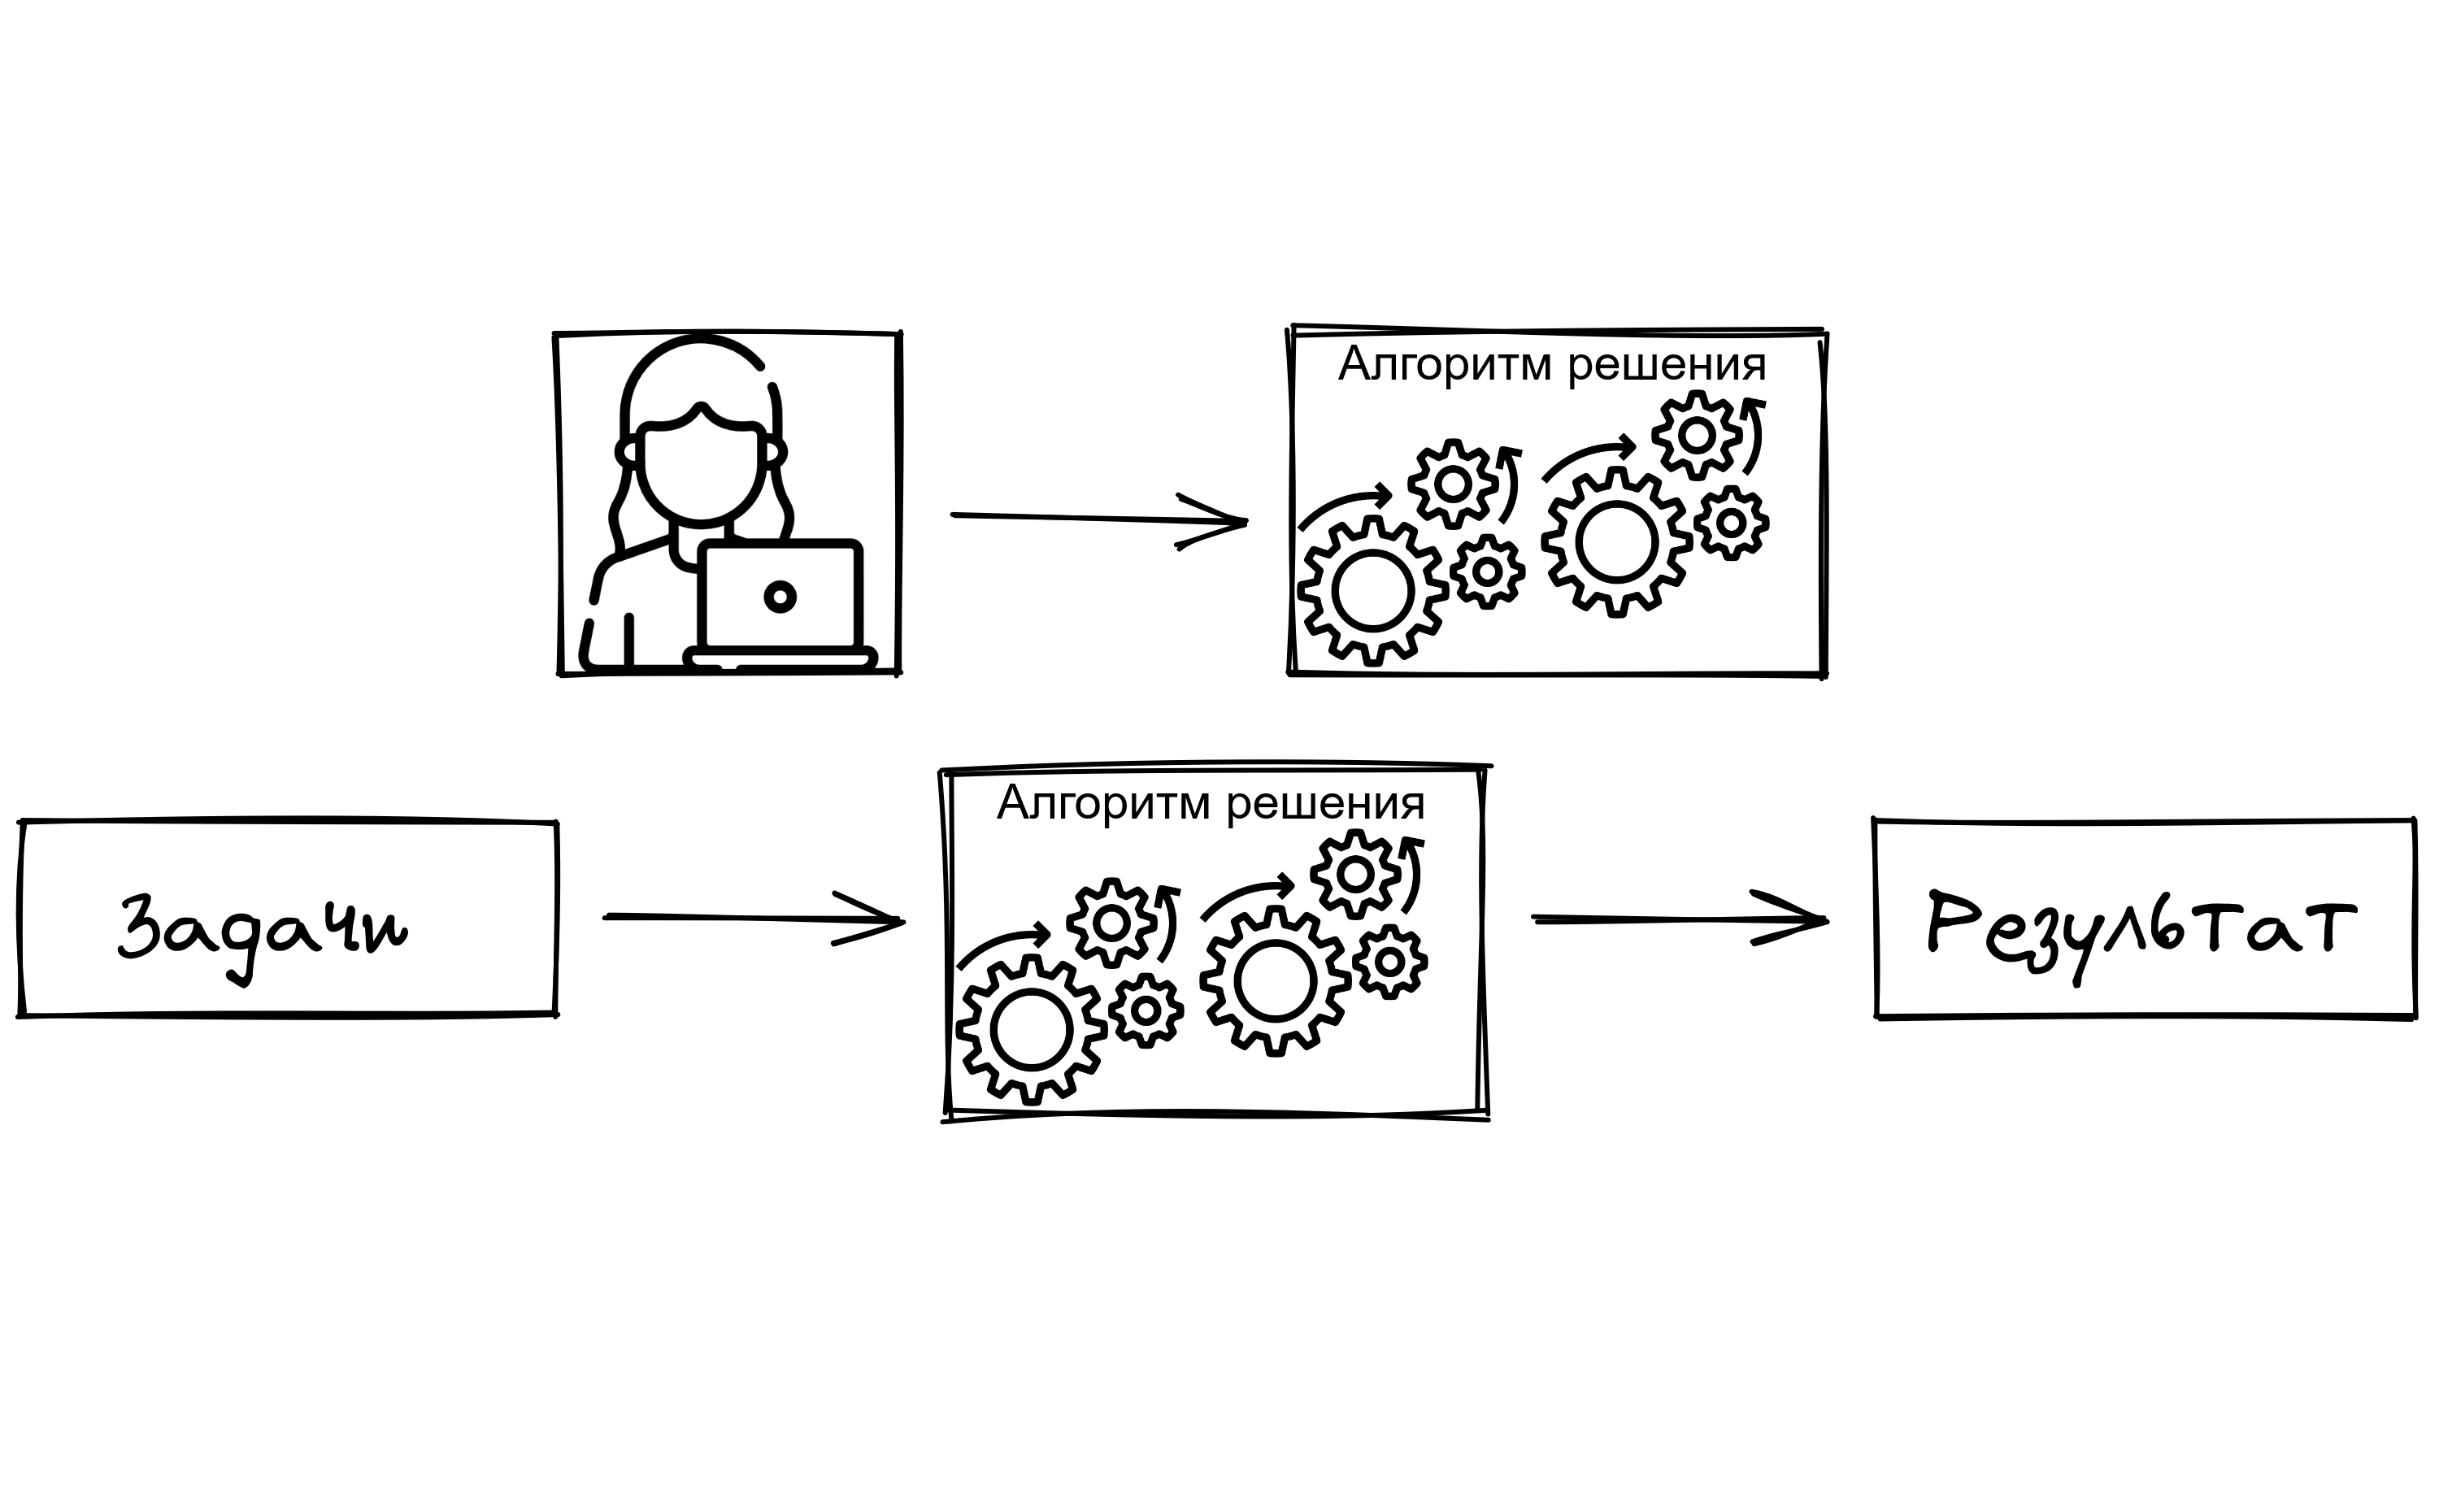
\includegraphics[width=\linewidth]{graphs/fig19_1.jpg}
        \end{column}
        \pause
        \begin{column}{.49\linewidth}
            \centering
            Machine Learning
            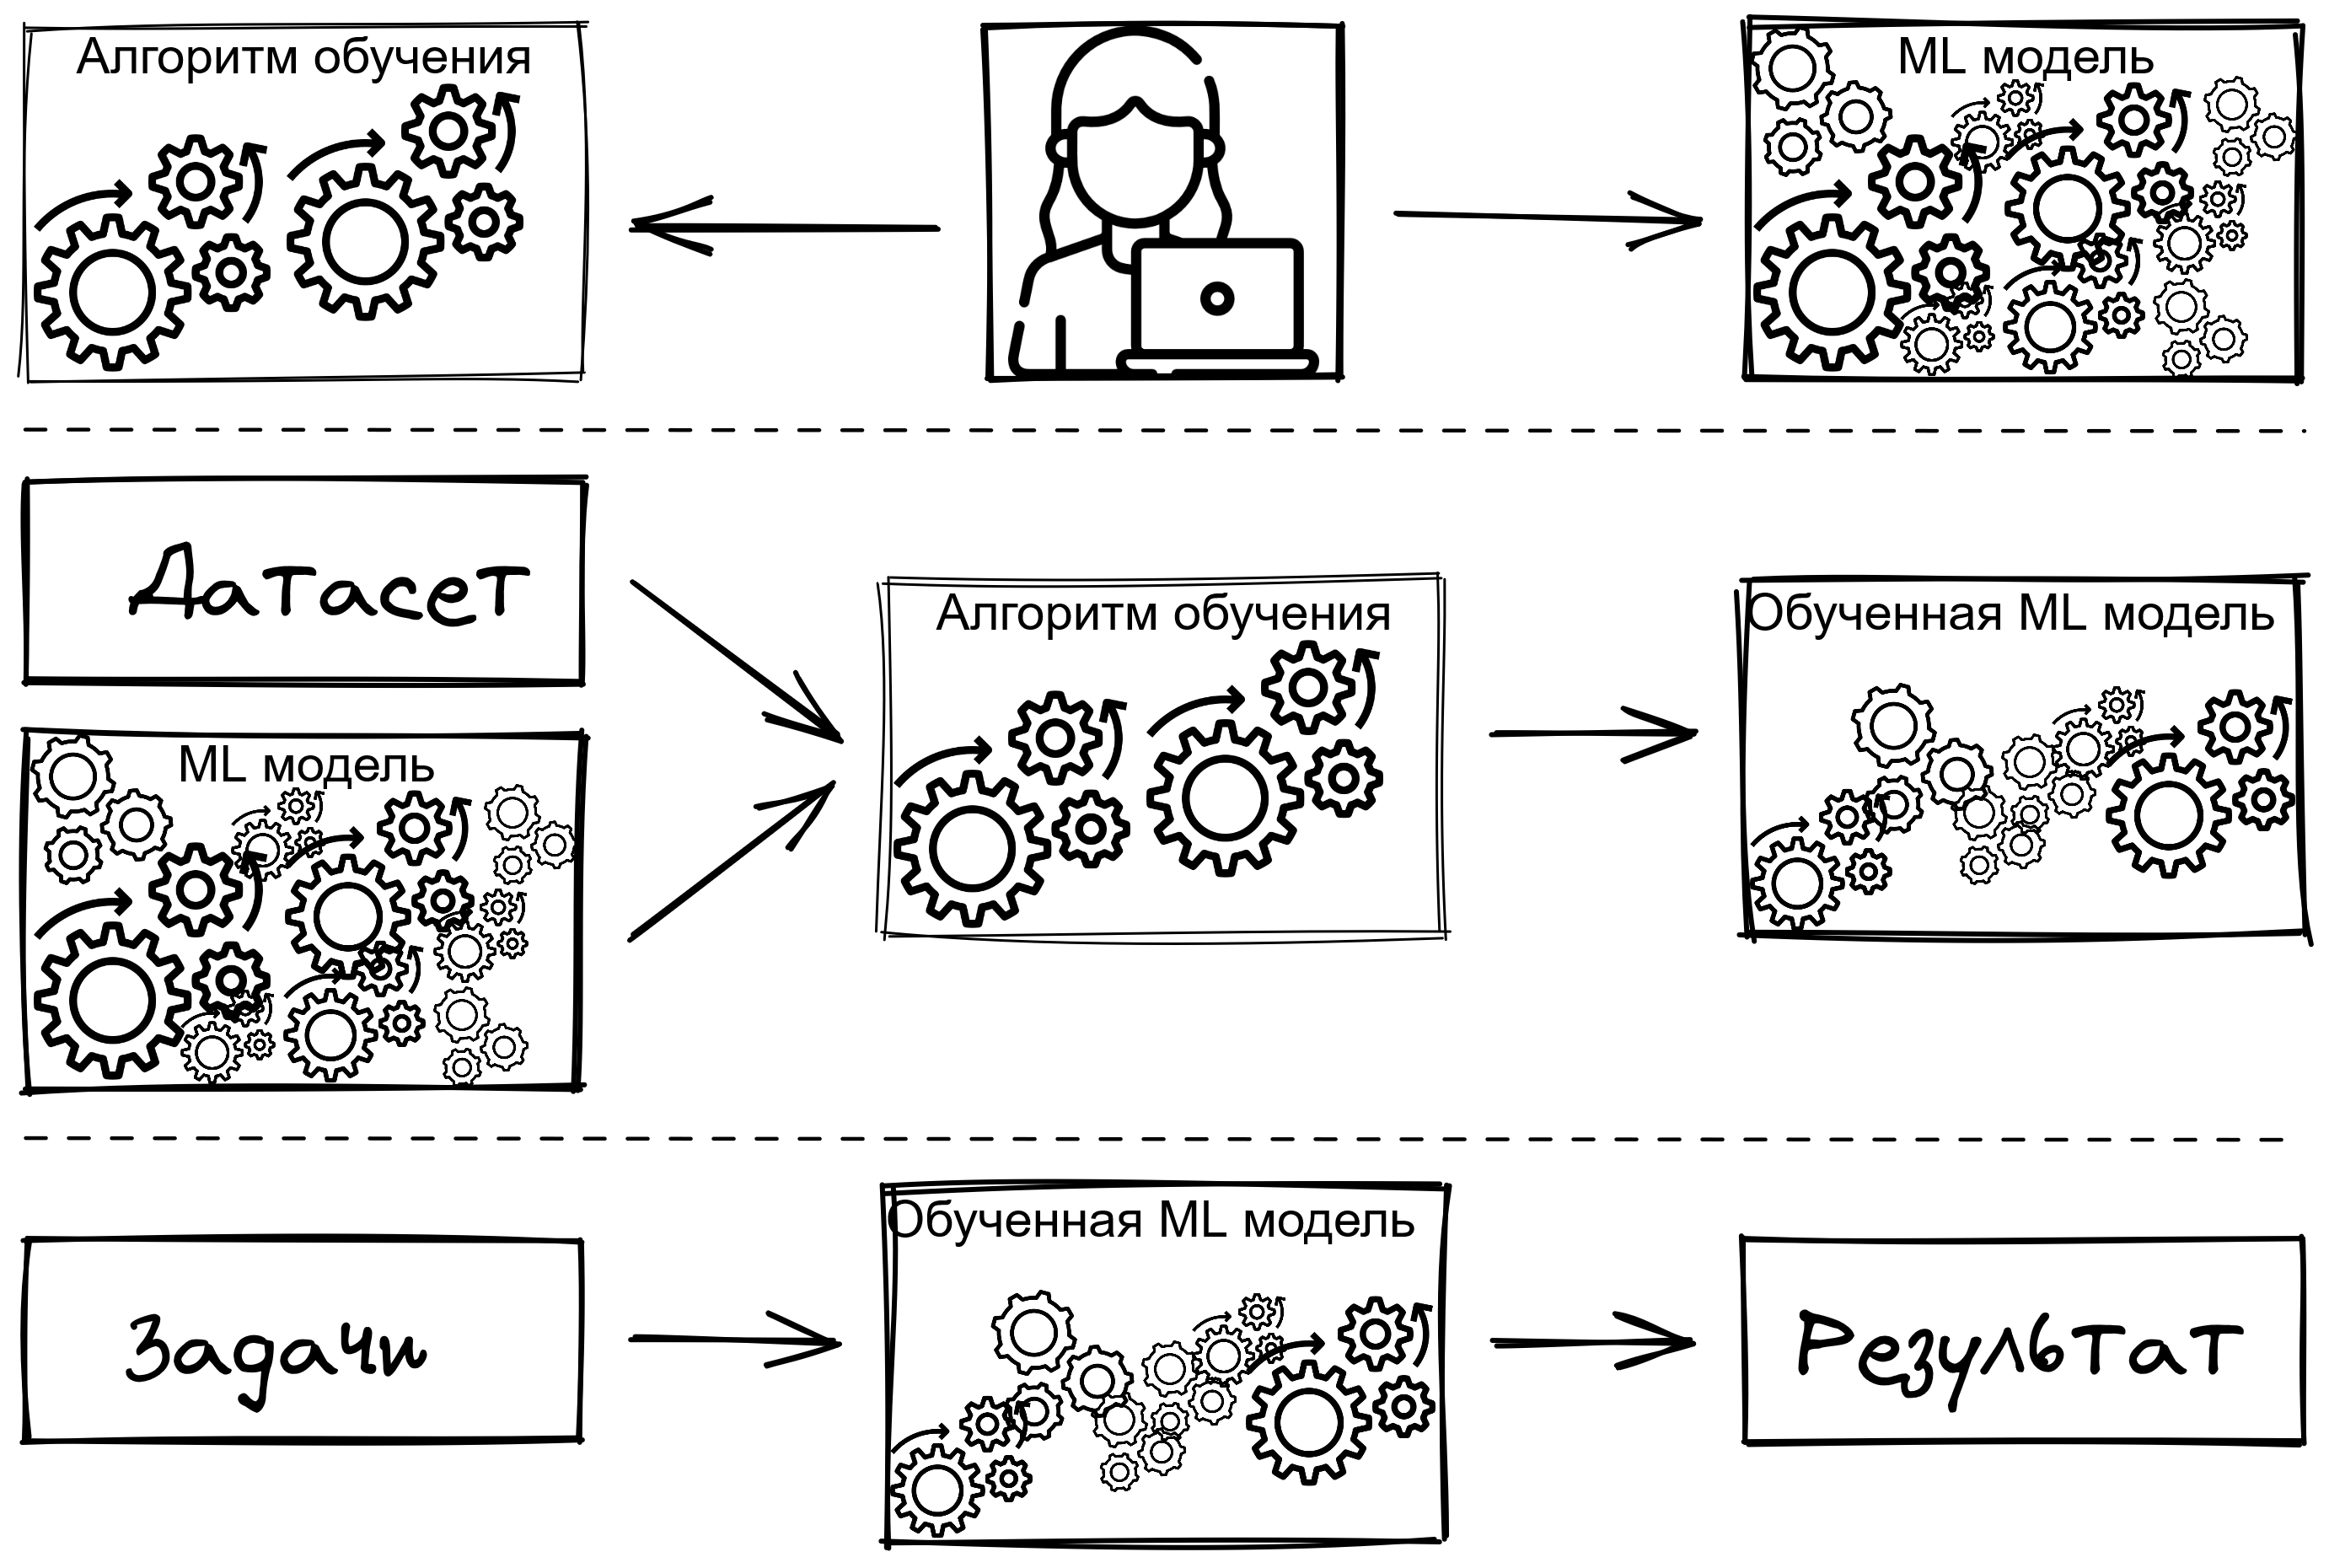
\includegraphics[width=\linewidth]{graphs/fig19_2.jpg}
        \end{column}
    \end{columns}
\end{frame}

\begin{frame}{Когда применим ML?}
    Смысл от применения машинного обучения появляется, когда:
    \begin{outline}
        \1 мы не можем создать точный алгоритм решения задачи, потому что
        слишком мало понимаем лежащие в её основах процессы и
        \textbf{не можем построить} точную модель этих процессов
        \pause
        \1 или модель есть, но ее полный расчет невозможен ввиду вычислительных
        ограничений (как в квантовой химии) 
        \pause
        \1 но при этом мы можем собрать \textbf{достаточное} количество данных с примерами
        правильного и неправильного решения задачи
    \end{outline}
\end{frame}

\begin{frame}{Когда применим ML?}
    \begin{outline}
        \1 Модели машинного обучения пытаются \textbf{восстанавливать закономерности} на
        основе \textbf{данных}, а не исходя из понимания природы или здравого смысла
        \1 ``Золотое'' правило машинного обучения
    \end{outline}
    \begin{center}
        
\includegraphics[width=.49\linewidth]{graphs/fig20.jpg} \\
        garbade in --- garbage out
    \end{center}
\end{frame}

\begin{frame}{Почему применять ML сложно?}
    \begin{outline}
        \1 Машинное обучение находится на стыке матстатистики, программирования и
        вычислительной математики (численной оптимизации)
        \pause
        \1 ML алгоритмы являются статистическими по своей сути, поэтому при их
        использовании необходимо допущение об ``устойчивости'' процесса
        \pause
        \1 Суть и основная проблема машинного обучения: модель учится на некоторой
        конечной выборке данных, а мы хотим чтобы она работала в будущем, на
        новых данных
        \pause
        \1 Из-за этого возникают специфичные проблемы: недообучение,
        переобучение, протечки
        \pause
        \1 А также используются специфичные способы проверки работоспособности модели
    \end{outline}
\end{frame}

\begin{frame}{Если же это не учитывать, то\ldots}
    \centering
    \ldots результат выйдет примерно таким \\
    
\includegraphics[width=.34\linewidth]{graphs/fig21.jpg}
\end{frame}

\begin{frame}{История}
    \centering
    \includegraphics[width=\linewidth]{graphs/fig22.jpg} \\
    82 года истории исследований AI
\end{frame}

\begin{frame}{Первая зима искусственного интеллекта}
    \begin{columns}
        \begin{column}{.49\linewidth}
            \centering
            \includegraphics[width=.75\linewidth]{graphs/fig23_1.jpg} \\
            Фрэнк Розенблатт и первый в мире нейрокомпьютер (1958г.)
        \end{column}
        \pause
        \begin{column}{.49\linewidth}
            \centering
            \includegraphics[width=.55\linewidth]{graphs/fig23_2.jpg} \\
            и книга, которая разрушила его работу (1962г.)
        \end{column}
    \end{columns}
\end{frame}

\begin{frame}{Вторая зима искусственного интеллекта}
    \centering
    \includegraphics[width=\linewidth]{graphs/fig22.jpg}
\end{frame}

\begin{frame}{Уроки истории}
    \large
    \begin{outline}
        \1 Искусственные нейросети были изобретены не несколько лет назад, а еще в 50-е
        \1 Со времени своего изобретения они прошли несколько пиков популярности и забвения
        \1 Почему тогда сейчас нейронные сети и машинное обучение опять на хайпе?
    \end{outline}
\end{frame}

\begin{frame}{Наступил 2012 год}
    \centering
    \includegraphics[width=.85\linewidth]{graphs/fig24.jpg}
\end{frame}

\begin{frame}{Больше данных}
    \centering
    \includegraphics[width=\linewidth]{graphs/fig25.jpg}
\end{frame}

\begin{frame}{Больше размеченных данных}
    \centering
    \includegraphics[width=\linewidth]{graphs/fig26.jpg}
\end{frame}

\begin{frame}{Больше размеченных данных}
    \centering
    \includegraphics[width=.97\linewidth]{graphs/fig27.jpg}
\end{frame}

\begin{frame}{Больше размеченных данных}
    \begin{outline}
        \1 C 2010 года проводится ILSVRC --- ImageNet Large Scale Visual
        Recognition Competition
        \1 Это соревнование, помимо открытого доступа к большому датасету
        ImageNet, дало научному сообществу простой способ сравнивать
        различные модели, что сильно ускорило прогресс в области компьютерного зрения
    \end{outline}
\end{frame}

\begin{frame}{Много данных --- тоже проблема}
    \begin{columns}
        \begin{column}{.49\linewidth}
            \centering
            \includegraphics[width=.8\linewidth]{graphs/fig28_1.jpg} \\
            70е: нет эффективных алгоритмов
        \end{column}
        \pause
        \begin{column}{.49\linewidth}
            \centering
            \includegraphics[width=.6\linewidth]{graphs/fig28_2.jpg} \\
            00е: расчеты будут идти вечность
        \end{column}
    \end{columns}
\end{frame}

\begin{frame}{Геймеры спасают науку о данных}
    \centering
    \includegraphics[width=.83\linewidth]{graphs/fig29.jpg}
\end{frame}

\begin{frame}{GPU - Graphics Processing Unit}
    \centering
    \includegraphics[width=.74\linewidth]{graphs/fig30.jpg}
\end{frame}

\begin{frame}{Конкуренция --- это прекрасно}
    \begin{columns}
        \begin{column}{.49\linewidth}
            \centering
            \includegraphics[width=\linewidth]{graphs/fig31_1.jpg}
        \end{column}
        \begin{column}{.49\linewidth}
            \centering
            \includegraphics[width=\linewidth]{graphs/fig31_2.jpg}
        \end{column}
    \end{columns}
\end{frame}

\begin{frame}{GPU vs. CPU}
    \centering
    \includegraphics[width=.92\linewidth]{graphs/fig32.jpg}
\end{frame}

\begin{frame}{Ученые любят GPU}
    \centering
    \includegraphics[width=\linewidth]{graphs/fig33.jpg}
\end{frame}

\begin{frame}{Глубокое обучение шагает по планете}
    \centering
    \includegraphics[width=.75\linewidth]{graphs/fig34.jpg}
\end{frame}

\begin{frame}{Глубокое обучение шагает по планете}
    \centering
    \includegraphics[width=.8\linewidth]{graphs/fig35.jpg} \\
    Количество принятых статей на конференцию NeurIPS
\end{frame}

\begin{frame}{Глубокое обучение шагает по планете}
    \centering
    \includegraphics[width=.6\linewidth]{graphs/fig36.jpg}
\end{frame}

\begin{frame}{Суть машинного обучения}
    \centering
    \includegraphics[width=.4\linewidth]{graphs/fig37.jpg}
\end{frame}

\begin{frame}{Следующее занятие}
    Через неделю:
    \begin{outline}
        \1 Обсудим задачи, которые решает машинное обучение
        \1 План курса
        \1 Приступим к практике
    \end{outline}
    Потребуются ноутбуки и google-аккаунт!
\end{frame}
\end{document}
